%Create document as an extraarticle and 12th fontsize
\documentclass[a4paper,12pt]{article}
\usepackage[utf8]{inputenc}
\renewcommand{\rmdefault}{ftm}
%Text position on a page
\usepackage[margin=1in, left=3cm,right=1cm, top=2cm,bottom=2cm,bindingoffset=0cm]{geometry}
\usepackage{setspace}
\onehalfspacing

%Creating titles views as you need
\usepackage{titlesec}

\titleformat*{\section}{\normalfont\normalsize\large}
\titleformat*{\subsection}{\normalfont\normalsize}
\titleformat*{\subsubsection}{\normalfont\normalsize}

\titlespacing{\section}{5ex}{*4}{*1}
\titlespacing{\subsection}{5ex}{*4}{*1}
\titlespacing{\subsubsection}{5ex}{*4}{*1}

%Creating itemizating without spaces between lines
\usepackage{enumitem}
\setlist[itemize]{noitemsep, topsep=0pt}

%intext references parameters
\usepackage[hidelinks, linktoc=all, backref=page, russian]{hyperref}
\usepackage{indentfirst}
\usepackage[russian]{babel}
\usepackage{subcaption}
\captionsetup[subfigure]{justification=centering}
\usepackage{wrapfig}
\usepackage[font=small, justification=centering]{caption}
\usepackage{abstract}
\usepackage{mathtools}
\usepackage{fancyhdr}
\usepackage{bbm}
\usepackage{bm}
\usepackage{cleveref}
\usepackage{xcolor}
\usepackage{hyperref}
\definecolor{linkcolor}{HTML}{799B03}
\setlength{\parskip}{0.1cm} 

%Each paragraph start option
\usepackage{indentfirst}  
\setlength{\parindent}{5ex}
%Pictures label option
\RequirePackage{caption}
\DeclareCaptionLabelSeparator{defffis}{ -- }
\captionsetup{justification=centering,labelsep=defffis}
\usepackage{graphicx} % Used to insert images
\usepackage{adjustbox} % Used to constrain images to a maximum size 
\usepackage{color} % Allow colors to be defined
\usepackage{enumerate} % Needed for markdown enumerations to work
\usepackage{geometry} % Used to adjust the document margins
\usepackage{amsmath} % Equations
\usepackage{amssymb} % Equations
\usepackage[mathletters]{ucs} % Extended unicode (utf-8) support


\usepackage{grffile} % extends the file name processing of package graphics 
% to support a larger range 
% The hyperref package gives us a pdf with properly built
% internal navigation ('pdf bookmarks' for the table of contents,
% internal cross-reference links, web links for URLs, etc.)
\usepackage{longtable} % longtable support required by pandoc >1.10
\hypersetup{pdfstartview=FitH,  linkcolor=black, colorlinks=true}



\setcounter{page}{5}
\begin{document}
	\def\figurename{Рисунок}
	\clearpage
	\setcounter{tocdepth}{3}
	
\begin{center}
	\large Аннотация
\end{center}



Выполнение любых алгоритмов подразумевает строгий контроль входных параметров. Не являются исключениями и алгоритмы, основанные на возможности некоторой физической системы находиться в когерентной суперпозиции двух собственных состояний. В данной дипломной работе описан процесс разработки программно-аппаратного комплекса по эффективной корректировке исходных состояний сверхпроводящих кубитов. Созданное устройство, используя алгоритмы машинного обучения, считывает и распознаёт текущее квантовое состояние и при необходимости переводит его в нужное. Весь цикл занимает время, существенно меньшее времён декогеренции и релаксации.

Выпускная квалификационная работа изложена на 40 страницах, содержит 33 рисунка, список использованных источников из 28 наименований. 
	\clearpage
	\renewcommand\contentsname{\centering\large Содержание}
\tableofcontents

	\clearpage
	\begin{center}
	\large{Введение}
\end{center}
\addcontentsline{toc}{section}{Введение}%\dotfill}

В 1982 году Ричард Филлипс Фейнман заметил, что моделирование даже самой простой квантово-механической системы требует колоссальных вычислительных ресурсов обычного классического компьютера, и высказал идею о том, что для решения таких задач можно использовать вычислительные системы, основанные на принципах квантовой механики  \cite{Feynman1982}.

Своё продолжение эта идея нашла в работах американского математика и информатика Питера Шора в 1995 году \cite{Shor1995}. Был разработан так называемый алгоритм Шора, решающий экспоненциально сложную с точки зрения подхода классического компьютера задачу факторизации больших чисел (разбиения их на простые сомножители). Эта задача нисколько не является абстрактной. На невозможности классического компьютера факторизовывать большие числа современная криптография построила почти всю систему защиты информации.

Ещё одно интересное применение квантовых принципов вычисления было найдено в виде  так называемого алгоритма Гровера (GSA- grover search algorithm \cite{Grover1996}). Это решение задачи подбора, т.е. решение уравнения вида $f(x_1,x_2 ... x_n)=1$, где $f(x_1,x_2 ... x_n)$ есть некоторая булева функция многих переменных. Проще говоря, нужно подобрать такую комбинацию  $\{x_i\}$, для которой условие выполняется. Классический компьютер требует последовательного перебора всех $N=2^n$ возможных вариантов и, соотвественно, решает эту задачу за $2^n$ временных единиц. Используя же принципы квантовой механики GSA, решает эту задачу за $\frac{\pi}{4}\sqrt{2^n}$ временных единиц. 

Всё это показывает, что создание универсального квантового компьютера позволит наиболее рационально подойти к целому ряду вопросов, связанных с моделированием сложных систем, защитой и контролем информации, подбором включений для создания материалов с заданными свойствами, подбором компонентов лекарств и т.д. 

Очевидно, что для корректного выполнения таких задач необходимо уметь приготавливать квантовые состояния, выполнять на них логические операции и считывать результат. Этой теме и посвящена данная работа. 

	\clearpage
	\section{Аналитический обзор литературы}
\subsection{Квантовая динамика двухуровневой системы}
\subsubsection{Формализм оператора плотности}

Согласно постулатам квантовой механики любое квантовое состояние может быть представлено в виде суперпозции (линейной комбинации) состояний называемых собственными:

\begin{equation}
\label{superposition}
|\psi(t)\rangle = \sum_n C_n(t)|\psi_n(t)\rangle,
\end{equation}
\\
\noindent где $C_n$ есть нормированные на единицу амплитуды вероятности обнаружить систему в одном из состояний $|\psi_n(t)\rangle$. Для вычисления математического ожидания некоторой физической величины ей в соответствие ставится линейный эрмитовый оператор:

\begin{eqnarray}
\begin{split}
\label{operator}
\langle A \rangle _t = \langle \psi(t) | A |\psi(t)\rangle = &
  \sum_{n,m} C_m(t) C_n(t) A_{nm} = \\
&= \sum_{n,m} \rho_{n,m}(t) A_{n,m} = Tr (\rho(t), A).
\end{split}
\end{eqnarray} 

Здесь введено дополнительное обозначение: $\rho_{n,m}(t)= C^*_n(t)C_m(t)$  называемое матричным элементом оператора плотности. Смысл его использования становится ясен при рассмотрении систем, для которых нахождение одном из чисто квантовых состояний имеет статистический характер. Введя вероятности $P_i(t)$ нахождения системы в чистых состояниях, можно задать наиболее общее определение матрицы плотности:

\begin{equation}
	\rho = \sum_i P_i(t) |\psi_i\rangle\langle\psi_i|
\end{equation} 

Рассмотрение вычисления математического ожидания для смешанного состояния, когда система изначально может находиться в одном из $|\psi_i(t)\rangle$, даёт следующий результат:

 \begin{equation}
 \begin{split}
 \label{operator}
 \langle A \rangle _t = \sum_i \langle \psi_i(t) | A |\psi_i(t)\rangle = 
 \sum _i \sum_{n,m} P_i(t )C_m(t)& C_n(t) A_{nm} = \\
 &= \sum_{n,m} \rho_{n,m}(t) A_{n,m} = Tr (\rho(t), A).
 \end{split}
 \end{equation} 
 
 Итоговое выражение с точки зрения математики не изменилось, но теперь оно означает проведение сразу двух усреднений. Одно из них учитывает квантово-механическое поведение системы, а другое стохастические процессы, происходящие при взаимодействии с окружением.
 
  Матрица плотности обладает следующими важными свойствами:
 \begin{itemize}
 	\item[a)] $Tr (\rho) = 1$. Это следует из определения;
 	\item[б)] $\rho^2 = \rho$ в случае чистых состояний. Действительно, тогда собственные значения оператора удовлетворяют условию $\rho_i = \rho_i^2$, а значит, из всех возможных квантовых состояний реализует только одно;
 	\item[в)] $Tr(\rho^2) \le 1$. Равенство выполняется в случае чистых состояний. Величину $Tr(\rho^2)$ можно использовать, как характеристику чистоты состояния. 
 \end{itemize} 

  Диагональные элементы матрицы плотности дают информацию о вероятностях обнаружить систему в одном из собственных состояний. Недиагональные элементы никак не влияют на значения математического ожидания наблюдаемых, однако они содержат в себе информацию о когерентности системы. С точки зрения измерения, если они равны нулю, это означает, что не существует такой наблюдаемой, в собственном состоянии которой находится система. Измерения будут давать результаты соответствующие разным собственным состояниям с вероятностями, определяемыми стохастическими процессами связи с окружением.Исключение составляет случай, когда один из диагональных элементов равен единице. 
  
  
  
  \subsubsection{Вектор Блоха и сфера Блоха}
  
  Для любой двухуровневой системы матрица плотности выступает в виде удобной и наиболее общей интерпретации состояния квантовой системы. Так, с её помощью можно дать дополнительное наглядное описание квантового состояния. Любая матрица 2х2 (в том числе и матрица плотности) может быть разложена в линейную комбинацию из единичной матрицы и матриц Паули, имеющих следующий вид:
  
  \begin{equation}
  \sigma_x = \begin{pmatrix} 0 & 1 \\ 1 & 0 \end{pmatrix}; \sigma_y = 
  \begin{pmatrix} 0 & -i \\ i & 0 \end{pmatrix}; \sigma_z = \begin{pmatrix} 1 & 0 \\ 0 & -1 \end{pmatrix};
  \end{equation}
 
  Используя это разложение, можно переписать матрицу плотности следующим образом:
    
\begin{equation}
\label{den_param}
\tag{6}
\rho = \frac{1}{2} \begin{pmatrix}1+R_z & R_x - iR_y \\ R_x + i R_y& 1-R_z\end{pmatrix} = \frac{1}{2}(\mathbb{I}+R_x\sigma_x+R_y\sigma_y+R_z\sigma_z) = \frac{1}{2}\vec R \cdot \vec{\sigma}
\end{equation}

Из условия, что $Tr(\rho^2)\le Tr(\rho)$ следует что:

\begin{equation}
\tag{7}
\begin{split}
Tr (\rho^2) = Tr\frac{1}{4} &
\begin{pmatrix}
(1+R_z)^2+ R_x^2+ R_y^2 & 2(R_x-iR_y) \\ 2(R_x+iR_y)& (1-R_z)^2+R_x^2+R_y^2
\end{pmatrix} = \\
&= \frac{1}{2}(1+R_x^2+R_y^2+R_z^2) \le 1
\end{split}
\end{equation}

Видно, что длина вектора $\vec{R}$ не может быть больше единицы. Поэтому его удобно использовать в наглядной интерпретации состояния системы, а именно, как показано на Рисунке 1, вектора внутри или на поверхности некоторой сферы, называемой сферой Блоха:
\begin{figure}[h]
	\centering
	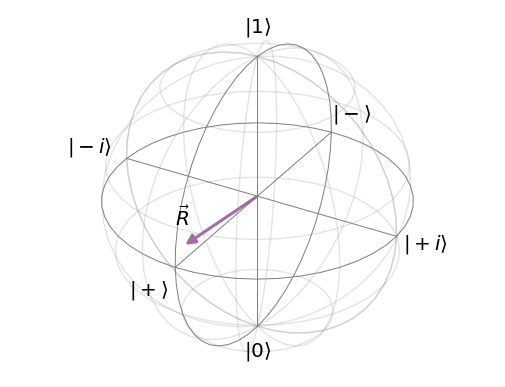
\includegraphics[width=0.4\linewidth]{pictures/Blochvect}
	\caption{Вектор Блоха на сфере Блоха}
	\label{fig:blochvect}
\end{figure}

Далее в работе вектор состояния двухуровневой системы будет обозначаться точками на сфере Блоха.

\subsubsection{Когерентная динамика двухуровневой системы}\label{cohdin}

Унитарная эволюция любой квантовой системы определяется её гамильтонианом, что следует напрямую из уравнения Шрёдингера. Для гамильтониана двухуровневой системы можно повторить приём, использованный в выражении (\ref{den_param}) :

\begin{equation}
\label{Ham}
\tag{8}
\hat H = \frac{\hbar}{2}(\omega_0\hat{\mathbb{I}}+\omega_1\hat\sigma_x+\omega_2\hat\sigma_y+\omega_3\hat\sigma_z) = \frac{\hbar}{2}\vec{\omega}\cdot\vec{\sigma}
\end{equation}
\\

Компонента при $\hat{\mathbb{I}}$ зависит от выбора начала отсчёта энергии и потому может быть опущена. Аналогом уравнения Шрёдингера для матрицы плотности является уравнение Лиувилля-фон-Неймана \cite{Neumann1957}:

\begin{equation}
\tag{9}
\label{liuv}
i\hbar\frac{\partial\hat\rho}{\partial t}=[\hat H, \hat\rho ]
\end{equation}
\\  

Подстановка результатов вычислений (\ref{den_param}) и (\ref{Ham}) в это уравнение приводит к следующему результату:

\begin{equation}
\tag{10}
\dot {\vec R} = \vec \omega \times \vec R
\end{equation}
\\

Это уравнение движения для вектора состояния двухуровневой квантовой системы. Впервые было получено и решено в работе \cite{Feynman1963}. Решением уравнения является чистая прецессия вектора состояния вокруг вектора, соответствующего гамильтониану системы.

В качестве примера будет рассмотрена произвольная двухуровневая система, взаимодействующая с внешней электромагнитной волной. В отсутствии внешнего возбуждения гамильтониан двухуровневой системы:

\begin{equation}
\label{tlsham}
\tag{11}
\hat H = \frac{\hbar\omega_q}{2}(|0\rangle\langle0| - |1\rangle\langle1|) = \frac{\hbar\omega_q}{2}\sigma_z
\end{equation}
\\

Гамильтониан электро-магнитного возбуждения, дипольно связанного с двухуровневой системой есть:

\begin{equation}
\tag{12}
\hat H = \hbar A \cos(\omega_d t) \hat\sigma_x , 
\end{equation}

\noindent а итоговый гамильтониан системы имеет следующий матричный вид:

\begin{equation}
\tag{13}
\hat H = \frac{\hbar}{2}\begin{pmatrix} \omega_q & A(e^{i\omega_d t} + e^{-i\omega_d t})\\ A(e^{i\omega_d t} + e^{-i\omega_d t})& -\omega_q \end{pmatrix}
\end{equation}
\\

Для того чтобы сделать задачу стационарной необходимо перейти в систему координат, вращающуюся с частотой внешней волны, делается это следующим унитарным преобразованием:

\begin{equation}
\label{unittr}
\tag{14}
\hat U = e^{\frac{i}{\hbar}\omega_d t\sigma_z}  = \begin{pmatrix}
e^{\frac{i}{2}\omega_d t} & 0 \\0& e^{-\frac{i}{2}\omega_d t}
\end{pmatrix}
\end{equation}
\\

Новый Гамильтониан вычисляется по формуле, напрямую следующей из уравнения Шрёдингера:

\begin{equation}
\tag{15}
\label{rabres}
\tilde{\hat H} = \hat U \hat H \hat U^\dagger+i\dot{\hat U}\hat U^\dagger 
\end{equation}




\noindent и имеет вид (более подробное решение описано в \cite{Gu2017}):

\begin{equation}
\tag{16}
\tilde{\hat{H}} = \frac{\hbar}{2}
\begin{pmatrix}
	\omega_q - \omega_d & A\\
	A&			\omega_d - \omega_q 
\end{pmatrix}
\end{equation}
\\
Для получения этого результата было использовано так называемое приближение вращающейся волны. Плоско-поляризованная внешняя волна, представляется как суперпозиция двух волн с круговой поляризацией. Преобразование (\ref{unittr}) переводит в систему отсчёта, связанную с одной из двух волн. Считается, что вторая волна, имея в новой системе отсчёта нерезонансную частоту не вносит серьёзного вклада. Из выражения (\ref{rabres}) видно, что состояние системы под действием внешней волны будет вращаться вокруг направления вдоль оси $X$ на сфере Блоха, как показано на Рисунке 2.
\begin{figure}[!h]
	\centering
	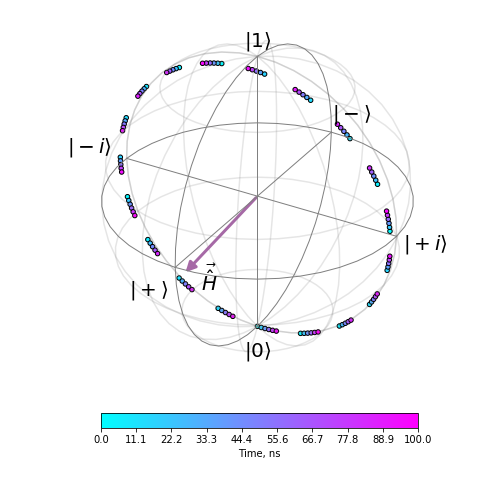
\includegraphics[width=0.4\linewidth]{pictures/Rabi}
	\caption{Динамика квантового состояния под воздействием внешнего излучения}
	\label{fig:rabi}
\end{figure}

Это периодическое изменение состояния называется осцилляциями Раби. Во-первых видно, что ввиду наличия некоторой отстройки частоты сигнала от частоты перехода в системе $(\omega_q - \omega_d \ne 0)$ система не может быть переведена в состояние $|1\rangle$ с вероятностью 100 \%. Во-вторых такая картина даёт информацию о необходимых длительностях сигналов переводящих систему в различные квантовые состояния. 

\subsubsection{Некогерентная динамика. Открытые системы}\label{neun}
Как уже было сказано, матрица плотности даёт возможность учитывать не только чисто квантовые особенности поведения системы, но и неунитарные процессы, происходящие из-за взаимодействия с классическим окружением \cite{Budini2009,Talkner2009}. Любая система в той или иной степени является открытой, т.е. взаимодействует с окружением. Гамильтониан в наиболее общем случае имеет вид:
\begin{equation}
\tag{17}
\hat H_{SE} = \hat H_S + \hat H_E + \hat H_I 
\end{equation} 	
Здесь $\hat H_S$ - гамильтониан системы, $\hat H_E$ - гамильтониан окружения и, наконец, $\hat H_I$ - гамильтониан их взаимодействия. Эволюция системы всё ещё определяется выражением (\ref{liuv}), но и гамильтониан матрица плотности в нём теперь отражают состояние системы вместе с окружением. Т.е. уравнение принимает вид:
\begin{equation}
\tag{18}
\label{rhose}
i\hbar\frac{\partial\hat\rho_{SE}}{\partial t}= [\hat H_{SE},\hat\rho_{SE}]
\end{equation}
\\

Для того чтобы представить уравнение (\ref{rhose}) в виде выражения, описывающего унитарную эволюцию системы с дополнительным слагаемыми отвечающим за неунитарную эволюцию необходимо сделать ряд последовательных приближений:
\begin{itemize}
	\item [a)] воздействие окружения на систему считается слабым возмущением. А само окружение представляется в виде набора бозонных мод, так что его гамильтониан имеет вид: $\hat H = \sum_n \hbar\omega_n \hat a^\dagger_n\hat a$;
	\item [б)] состояние окружения считается постоянным и равновесным. В этом случае эволюция системы и эволюция окружения - статистически-независимые процессы и матрицу плотности $\hat \rho_{SE}$ можно представить в виде $\hat \rho_{SE} = \hat \rho_{S}\otimes\hat\rho_E$;
	\item[в)] характерные времена изменения матрицы плотности системы считается существенно меньше  корреляционных времён, связанных с процессами внутри системы, так что эволюция матрицы плотности определяется только её текущим состоянием и никак не зависит от предшествующих; 
\end{itemize}	

Применение приближений для изменения вида уравнения ({\ref{liuv}}) - громоздкая процедура, она подробно описана в работе \cite{Vool2017}. В результате в нём появляются слагаемые, отвечающие за отличие эволюции системы от унитарной. Итоговое уравнение имеет форму Линдблада:
\begin{equation}
\tag{19}
\label{lindblad}
i\hbar \frac{\partial\hat\rho}{\partial t} = [\hat H,\rho] + \sum_n (2\hat L_a \hat \rho \hat L^\dagger_n - \{\hat L^\dagger_n\hat L_n,\hat \rho\})
\end{equation} 
\\

Здесь $\hat L_n$ и $\hat L^\dagger_n$ - операторы Линдблада, вид которых подбирается в каждой конкретной задаче. В них содержится информация о механизмах и скоростях рассматриваемых процессов. В качестве примера будет рассмотрено несколько вариантов неунитарной эволюции двухуровневой системы. 

Для первого примера вид оператора Линдблада имеет вид:
\begin{equation}
\tag{20}
\label{dephaseop}
\hat L = \hat L^\dagger = \sqrt{\gamma}\hat \sigma^\dagger\hat \sigma^-  = \sqrt{\gamma}\begin{pmatrix}
1&0\\0&0\
\end{pmatrix}
\\
\end{equation}

После подстановки уравнение (\ref{lindblad}) представляет собой матричное дифференциальное уравнение:
\begin{equation}
\tag{21}
\begin{pmatrix}
\dot\rho_{00} & \dot\rho_{01}\\\dot\rho_{10}&\dot\rho_{11}
\end{pmatrix} = \begin{pmatrix}
0&-\gamma\rho_{01}\\-\gamma\rho_{10}&0
\end{pmatrix}
\end{equation}

Его решение даёт следующий результат:
\begin{equation}
\tag{22}
\hat\rho(t) = \begin{pmatrix}
\rho_{00}(0)&\rho_{01}(0)e^{-\gamma t}\\ \rho_{10}(0)e^{-\gamma t}&\rho_{11}(0)
\end{pmatrix}
\end{equation}

Такой вид неунитарной эволюции называется чистой дефазировкой. В этом случае диагональные элементы остаются постоянными, а недиагональные экспоненциально убывают во времени, скорость затухания при это определяется параметром $\gamma$. Чистота состояния так же убывает экспоненциально:

\begin{equation}
\tag{23}
tr\hat\rho^2(t) = \rho_{00}^2(0) +\rho_{11}^2(0) + |\rho_{01}^2(0)|e^{-2\gamma t}
\end{equation} 

Динамика состояния в этом случае будет иметь вид изображённый на Рисунке 3:
	
\begin{figure}[h]
	\centering
	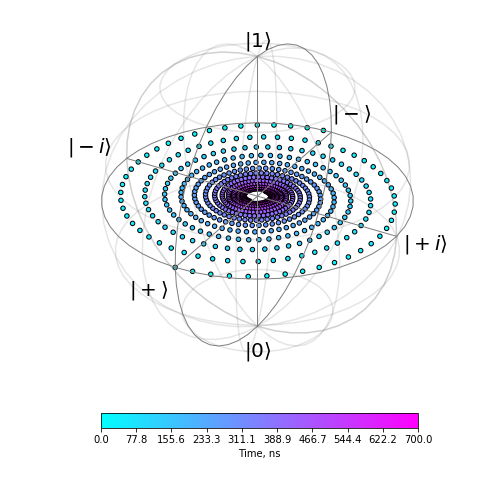
\includegraphics[width=0.4\linewidth]{pictures/Puredephase}
	\caption{Чистая дефазировка квантового состояния $|+\rangle$ на сфере Блоха}
	\label{fig:puredephase}
\end{figure}

В качестве второго примера будет рассмотрено влияние операторов Линдблада вида:
\begin{equation}
\label{relaxop}
\tag{24}
\begin{split}
&\hat L = \sqrt{\Gamma/2}\hat\sigma^\dagger- = \sqrt{\Gamma/2}
\begin{pmatrix}
0&1\\0&0
\end{pmatrix}\\
&\hat L^\dagger = \sqrt{\Gamma/2}\hat\sigma_- = \sqrt{\Gamma/2}
\begin{pmatrix}
0&0\\1&0
\end{pmatrix}
\end{split}
\end{equation}

Подстановка в (\ref{lindblad}) даёт матричное уравнение:
\begin{equation}
\tag{25}
\begin{pmatrix}
\dot\rho_{00}&\dot\rho_{01}\\
\dot\rho_{10}&\dot\rho_{11}
\end{pmatrix} =
\begin{pmatrix}
\Gamma\rho_{00}&-(\Gamma/2) \rho_{01}\\
-(\Gamma/2)\rho_{10} & -\Gamma\rho_{11}
\end{pmatrix},
\end{equation}

\noindent решение которого имеет вид:
\begin{equation}
\label{relax}
\tag{25}
\hat\rho(t) = 
\begin{pmatrix}
1-\rho_{11}(0)e^{-\Gamma t}& \rho_{01}(0)e^{(-\Gamma/2)t}\\
\rho_{10}(0)e^{(-\Gamma/2)t}&\rho_{11}(0)e^{-\Gamma t}
\end{pmatrix}
\end{equation}

С течением времени недиагональные элементы матрицы экспоненциально стремятся к нулю. На диагонали $\rho_{11}$, а $\rho_{00}$ - к единице. В дополнение к дефазировке, выражение (\ref{relax}) описывает так называемый процесс релаксации, т.е. передачи энергии из системы в связанное с ней окружение.
Интересно заметить, что эволюция берёт свой старт в чистом состоянии $|-\rangle$ и под действием неунитарных процессов, постепенно проходя через смешанное состояние, снова стремится к чистому состоянию $|0\rangle$. 

 Динамика квантового состояния $|-\rangle$ под действием оператора (\ref{relaxop}) представлена на Рисунке 4:

\begin{figure}[h]
	\centering
	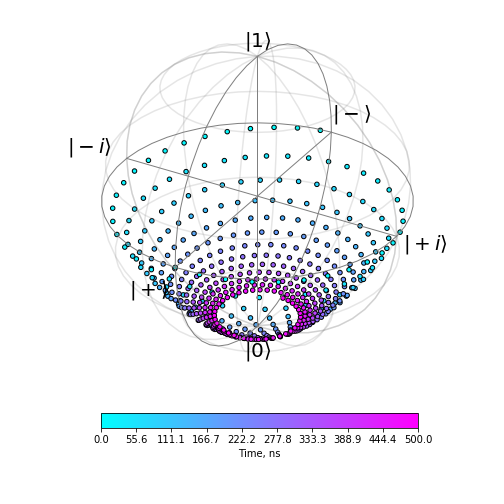
\includegraphics[width=0.4\linewidth]{pictures/Relaxation}
	\caption{Релаксация квантового состояния $|-\rangle$ на сфере Блоха}
	\label{fig:relaxation}
\end{figure}

Наконец, если учесть воздействие сразу двух операторов Линдблада (\ref{relaxop}) и (\ref{dephaseop}), решение уравнения (\ref{lindblad}) будет иметь вид:

\begin{equation}
\tag{26}
\hat \rho(t)= 
\begin{pmatrix}
\rho^e_{00}+(\rho_{00}(0)-\rho^e_{00})e^{-\Gamma t}&\rho_{01}(0)e^{-(\Gamma/2+\gamma)t}\\\rho_{10}(0)e^{-(\Gamma/2+\gamma)t} &
\rho^e_{11}+(\rho_{11}(0)-\rho^e_{11})e^{-\Gamma t}
\end{pmatrix}
\end{equation} 

Здесь $\rho^e_{00}$ и $\rho^e_{11}$ - некоторые равновесные заселённости квантовых состояний. Их значения могут быть расчитаны для каждой температуры T из соотношения: $\frac{\rho^e_{11}}{\rho^e_{00}}=e^{-\frac{\hbar\omega_q}{k_BT}}$.

Динамика квантового состояния в этом случае изображена на Рисунке 5: 
\begin{figure}[!h]
	\centering
	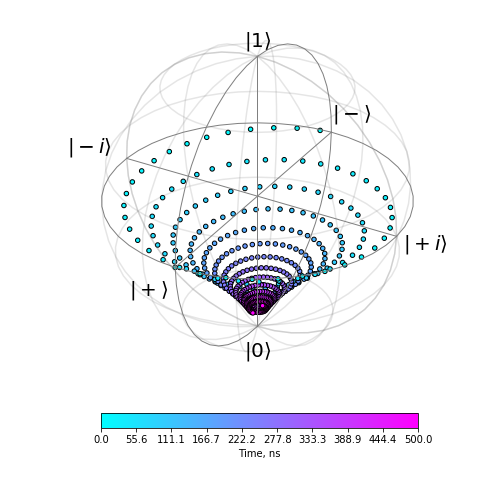
\includegraphics[width=0.4\linewidth]{pictures/Relaxdephase}
	\caption{Процессы релаксации и дефазировки квантового состояния $|-\rangle$ на сфере Блоха}
	\label{fig:relaxdephase}
\end{figure}

\subsection{Трансмон}\label{transmon}

На данный момент существует целый спектр физических реализаций двухуровневых систем \cite{Gershenfeld1997,Jaksch2000,Buluta2011}. Одним из наиболее развиваемых сильнейшими в мире лабораториями является направление, основанное на сверхпроводящих устройствах \cite{Yan2016,Martinis2009,DeGraaf2018}. Об одном из таких устройств и пойдёт речь в этой главе. 

Первично идея зарядового кубита была предложена в работе \cite{Nakamura1999}. Схема реализации представлена на Рисунке 6:
\begin{figure}[h]
	\centering
	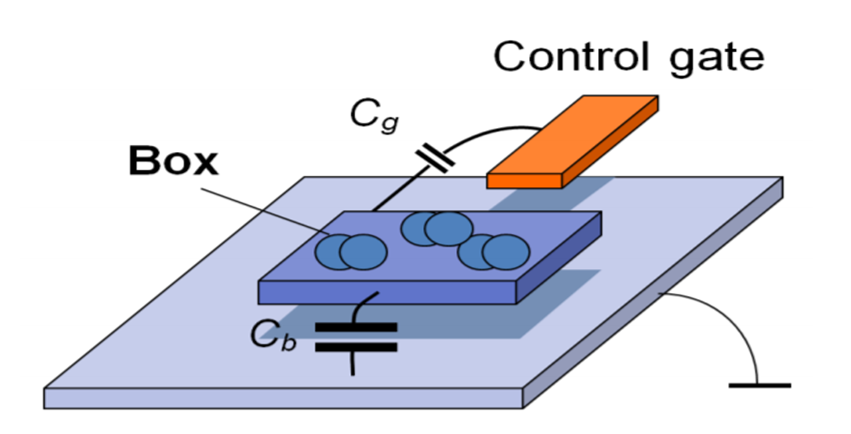
\includegraphics[width=0.6\linewidth]{pictures/chargequbit}
	\caption{Зарядовый кубит \cite{Shulga2017}}
	\label{fig:chargequbit}
\end{figure}

К небольшому сверхпроводящему островку (Box), ёмкостно связанному со сверхпроводящией плоскостью (землёй), подводится контролирующее напряжение (Control gate). При достижении низких температур число куперовских на островке квантуется.  С помощью изменения напряжения на Control gate можно получить ситуацию, когда состояния с разным числом куперовских пар на острове вырождаются. Вырождение снимается, если куперовские пары получают возможность тунелировать на землю за счёт эффекта Джозефсона \cite{Wendin2005}. Величина расщепления в первом приближении равна энергии, необходимой куперовской паре на тунелирование. Итоговый гамильтониан системы состоит из зарядового и Джозефсоновского вклада и может быть записан в виде:

\begin{equation}
\hat H = E_C (\hat n - n_g)^2 - E_J \cos {\hat \phi}, 
\label{cpb1}
\tag{27}
\\
\end{equation}

\noindent где $E_C = \frac{(2e)^2}{2C_q}$ - зарядовая энергия, а $E_J = \frac{\Phi_0 I_C}{2\pi}$ - Джозефсоновская энергия. Так же в выражении  (\ref{cpb1}) присутствуют операторы числа куперовских пар на островке - $\hat n_g$  и фазы волновой функции сверхпроводящего состояния $\hat \phi$. При низких температурах для них выполняется коммутационное соотношение: 

\begin{equation}
\label{commut}
\tag{28}
[\hat n, \hat \phi ] = i
\end{equation}

Используя (\ref{commut}) можно переписать гамильтониан (\ref{cpb1}) в виде:

\begin{equation}
\tag{29}
\label{cpb}
\hat H  = \sum_n [E_C(n-n_g)^2]|n\rangle\langle n| - \frac{E_j}{2}(|n\rangle\langle n+1|+|n+1\rangle\langle n|)]
\end{equation} 


На Рисунке 7 приведён результат численной диагонализации гамильтониана (\ref{cpb}) для разных соотношений $E_j/ E_c$. Полученные состояния являются функциями напряжения на Control gate (или заряда $n_g$).
\begin{figure}[h]
	\centering
	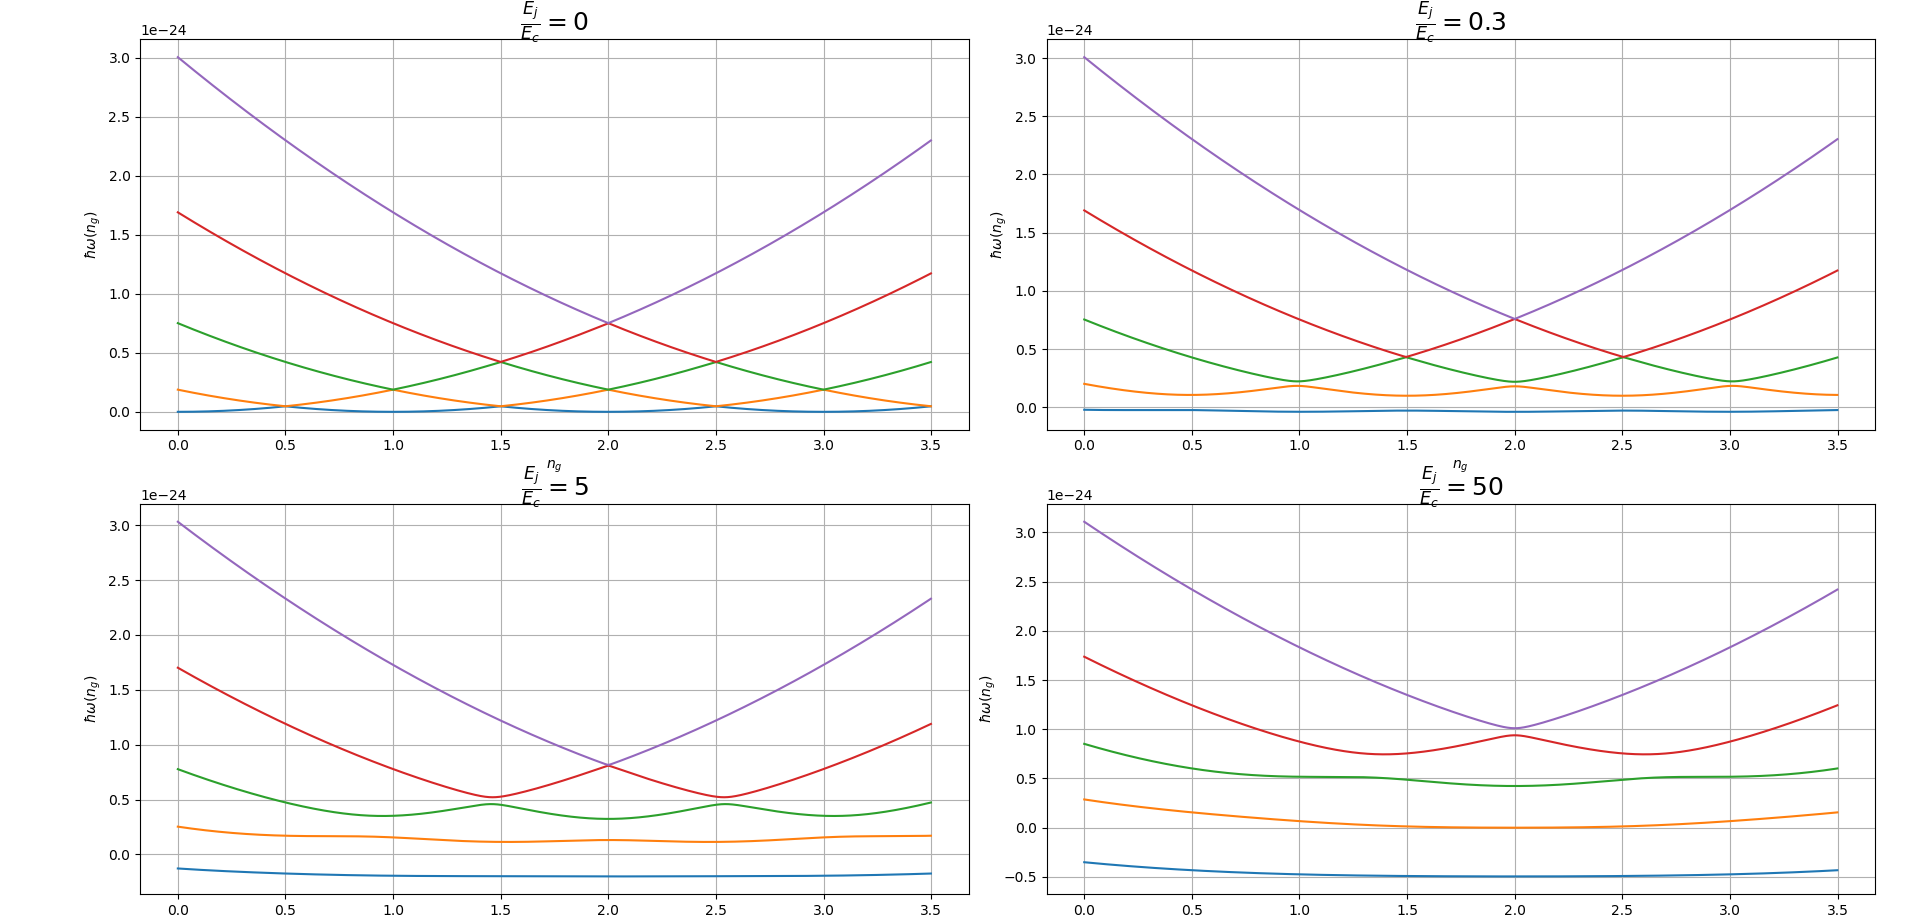
\includegraphics[width=0.9\linewidth]{pictures/cpb}
	\caption{Спектральные линии зарядового кубита}
	\label{fig:cpb}
\end{figure}

Видно, что в случае отсутствия Джозефсоновской энергии спектральные линии пересекаются. При её появлении вырождение снимается, но до тех пор пока преобладает зарядовая энергия наблюдается сильная зависимость энергии состояний от наведённого заряда, что, как было показано в (\ref{neun}) ведёт к дополнительной дефазировке.  Проблема была решена в работе \cite{Koch2007}. Был создан кубит-трансмон. С помощью большой шунтирующей ёмкости удалось  получить соотношение $\frac{E_J}{E_C}  \sim 50$ и избавиться таким образом от зарядовой дисперсии. Как видно из Рисунка 7, энергетическая структура в этом случае представляет собой неэквидистантные уровни ангармонического осциллятора. Из теории возмущения можно рассчитать поправки к частотам переходов:

\begin{equation}
\tag{30}
\begin{split}
&E_{01}= \sqrt{8E_JE_C}- E_C\\
&E_{12}= \sqrt{8E_JE_C}-2E_C
\end{split}
\end{equation}  

Частоту перехода в кубите так же можно контролировать, используя СКВИД \cite{Kleiner2004}. При манипуляции близкими по частоте перехода импульсами систему можно приближённо считать двухуровневой, а гамильтониан (\ref{cpb}) привести к виду:

\begin{equation}
\label{spinham}
\tag{31}
\hat H = -\frac{E_c}{2}(1-2 n_g)\hat \sigma_z - \frac{E_j}{2}\hat\sigma_x, 
\\
\end{equation}

\noindent который является полностью аналогичным виду гамильтониана самой распространённой двухуровневой системы, а именно одиночного спина $\frac{1}{2}$ в постоянном внешнем магнитном поле. 

\subsection{Трансмон связанный с резонатором} \label{transres}
Реализация любых вычислительных алгоритмов подразумевает возможность считать итоговый результат\cite{Wallraff2005}. Не являются исключением и алгоритмы квантовой информатики, которые базируются на возможности двухуровневой системы находиться в когерентной суперпозиции собственных состояний. 

Идея считывания квантовых состояний одиночных кубитов пришла из науки, которая называется квантовая электродинамика в полости (Cavity QED \cite{Blais2004}). Рассматривается система, изображённая на Рисунке 8:
\begin{figure}[h]
	\centering
	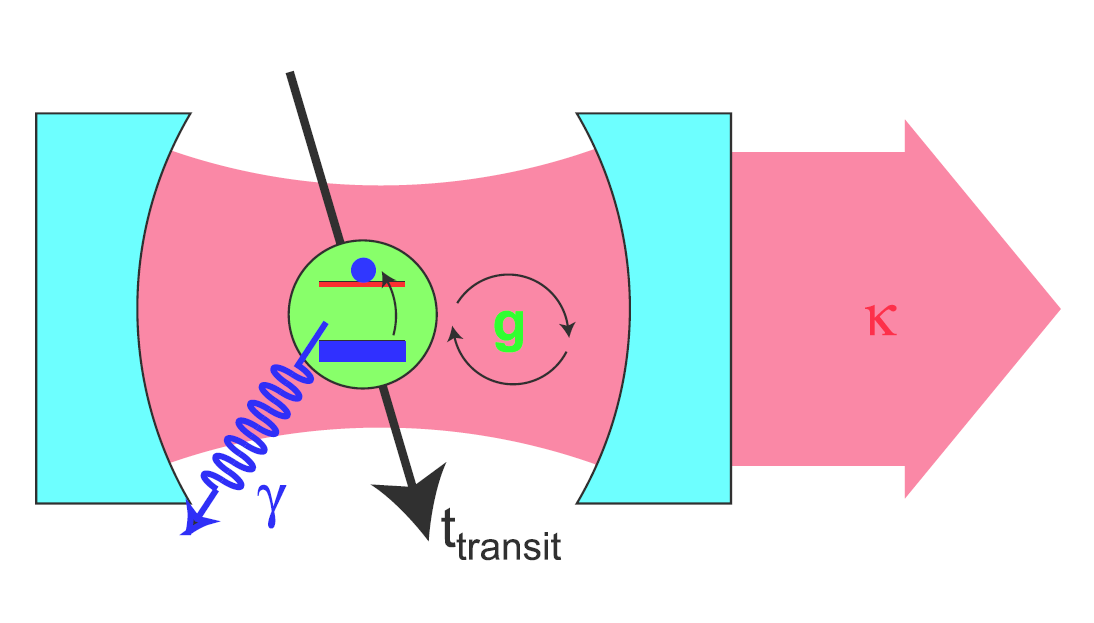
\includegraphics[width=0.5\linewidth]{pictures/qed}
	\caption{Система QED}
	\label{fig:qed}
\end{figure}

Она состоит из двух зеркал с распространяющимися между ними модами электромагнитного поля. Через зеркала пропускают пучок атомов. Эволюция системы определяется рядом параметров: $\gamma$ - декремент затухания заселённости возбуждённого состояния атома, определяется величиной связи атома с модами полей, в которые можно отдать энергию, $k$ - обратное время спонтанного излучения фотона из полости, определяется связью системы с континуумом мод за пределами полости, $g$ - сила связи моды полости с атомом, определяется величиной дипольного взаимодействия между ними. 

Естественно, что для создания универсального вычислительного устройства на основе механизмов квантовой механики необходима куда более масштабируемая система с идентичной энергетической структурой. Один из вариантов такой структуры рассмотрен в задаче квантовой электродинамике цепей (Circuit QED) и  изображён на  Рисунке 9.

Так же для наглядности на Рисунке 10 приведена оптическая фотография чипа, с физически реализованной системой.

Вместо системы зеркал здесь представлен участок передающей линии с разрывами на концах. Являясь по сути последовательностью LC- контуров, эта система представляет собой резонатор, частота которого определяется геометрическими параметрами. В область повышенной амплитуды поля помещён кубит Трансмон дипольно связанный с модой поля.


\begin{figure}[!h]
	\centering
	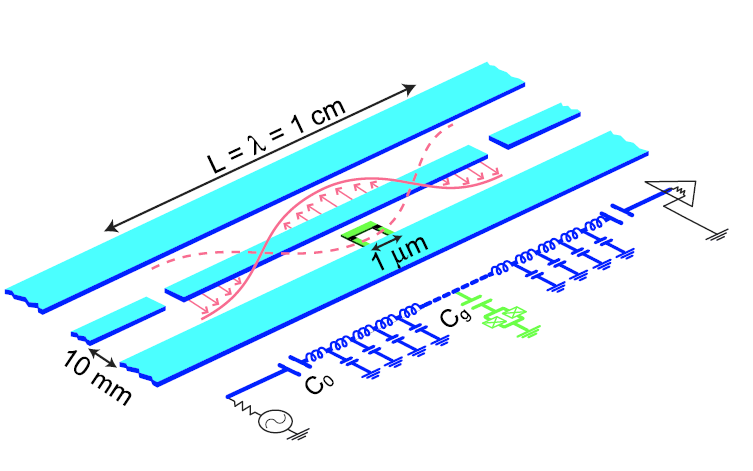
\includegraphics[width=0.5\linewidth]{pictures/qed1}
	\caption{Схема Circuit QED}
	\label{fig:qed1}
\end{figure}


\begin{figure}[h]
	\centering
	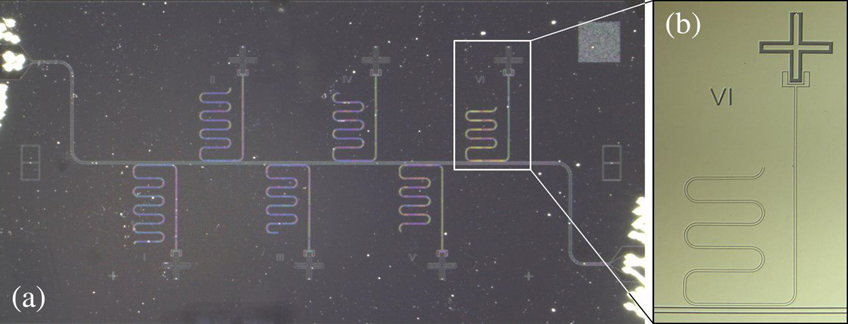
\includegraphics[width=0.5\linewidth]{pictures/chip}
	\caption{Чип с системой резонаторов и кубитов}
	\label{fig:chip}
\end{figure}

Эквивалентная электронная схема системы изображена на Рисунке 11:
\begin{figure}[!h]
	\centering
	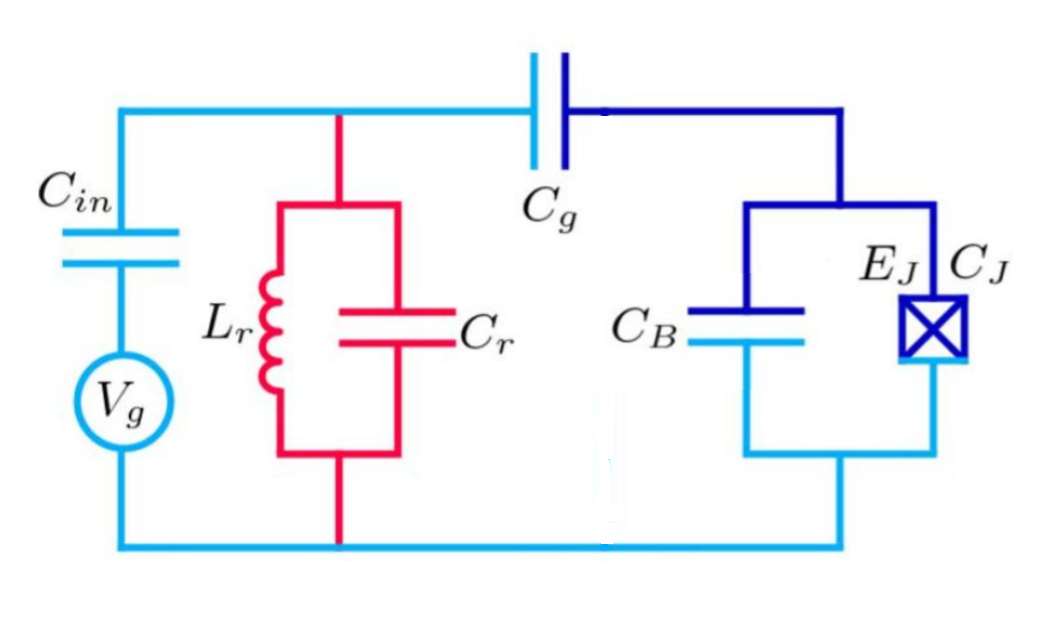
\includegraphics[width=0.5\linewidth]{pictures/electr}
	\caption{Эквивалентная электрическая схема кубита и резонатора}
	\label{fig:electr}
\end{figure}

Эволюция такой системы, а так же необходимость использования резонаторов для считывания квантовых состояний становится ясной при рассмотрении модели Джейнса-Каммингса \cite{Clarke2008}, согласно которой гамильтониан такой системы может быть представлен в виде:
\begin{equation}
\label{JCham}
\tag{32}
\hat H = \hbar\omega_r(\hat a ^\dagger \hat a +\frac{1}{2})-\frac{\hbar\omega_a}{2}\hat \sigma_z + \hbar g(\hat a^\dagger\hat\sigma^-+ \hat a\hat\sigma^\dagger) + \hat H_\gamma + \hat H_K
\\
\end{equation}

Здесь первое слагаемое - гамильтониан гармонического осциллятора, отвечающего резонаторной моде поля, второе - гамильтониан двухуровневой системы, третье - гамильтониан их взаимодействия. С физической точки зрения слагаемые $\hat a^\dagger\hat\sigma^-$  и $\hat a \hat\sigma^\dagger$ отвечают переходу возбуждения из кубита в резонатор и наоборот. $\hat H_k $ и $\hat H_\gamma$, как было указано ранее, отвечают за спонтанное излучение возбуждения из резонатора и атома соотвественно. Ввиду наличия связи состояния, отвечающие возбуждению в кубите или резонаторе, не являются собственными для оператора (\ref{JCham}). Происходит гибридизация и новые собственные состояния определяются, как линейная комбинация исходных $(\alpha|0,n\rangle+\beta|1,n-1\rangle)$.
Комплексные числа $\alpha$  и $\beta$ могут быть найдены из решения уравнения на собственные значения и собственные векторы указанного гамильтониана:
\begin{equation}
\tag{33}
\begin{split} 
\hat H &(\alpha|0,n\rangle+\beta|1,n-1\rangle) = E (\alpha|0,n\rangle+\beta|1,n-1\rangle) \iff\\
&\alpha\hbar\omega_r(n+\frac{1}{2})|0,n\rangle+\beta\hbar\omega_r(n-\frac{1}{2})|1,n-1\rangle - a\frac{\hbar\omega_q}{2}|0,n\rangle+\beta\frac{\hbar\omega_q}{2}|1,n-1\rangle + \\&\hbar g\sqrt{n}(\beta|0,n\rangle+\alpha|1,n-1\rangle)= E(\alpha|0,n\rangle+\beta|1,n-1\rangle)
\\
\end{split}
\end{equation}

Приравнивая коэффициенты при одинаковых состояния, можно получить:
\begin{equation}
\tag{34}
\begin{split}
&\alpha (\omega_r n +\frac{\Delta}{2}-\frac{E}{\hbar})+g\sqrt n \beta = 0\\
&\alpha g\sqrt n + (\omega_r n - \frac{\Delta}{2} - \frac{E}{\hbar})\beta  = 0 
\end{split}
\end{equation}

Здесь $\Delta = \omega_r - \omega_q$. Из определителя этой системы можно найти собственные значения гамильтониана:

\begin{equation}
\tag{35}
\frac{E}{\hbar}=\omega_r n \pm \sqrt{\frac{\Delta^2}{4}-g^2 n}
\\
\end{equation}

Как указывалось ранее практический интерес представляет режим работы системы, при котором $\Delta >>g$. В этом случае $n<<(\frac{\Delta}{2g})^2$ тогда второе слагаемое можно разложить в ряд Тейлора по параметру $(\frac{\Delta}{2g})^2$:

\begin{equation}
\tag{36}
\label{eighval}
\frac{E}{\hbar} = \omega_r n \pm \frac{\Delta}{2}(1- n \frac{g^2}{2\Delta^2})
\\
\end{equation}
В этом приближении выражения для собственных состояний системы имеют вид:
\begin{equation}
\tag{37}
\begin{split}
&|-,0\rangle = -\frac{g}{\Delta}|1,0\rangle + |0,1\rangle\\
&|+,1\rangle = |1,0\rangle + \frac{g}{\Delta}|0,1\rangle
\end{split}
\end{equation}
Наконец, подставив (\ref{eighval}) выражение для оператора числа возбуждений в системе:
\begin{equation}
\tag{38}
\hat n = -\frac{1}{2}(\hat \sigma_z +1)+\hat a^\dagger\hat a,
\end{equation}
\noindent можно получить:
\begin{equation}
\label{JChamD}
\tag{39}
\hat H_d = \hbar(\omega_r + \frac{g^2}{\Delta}\hat\sigma_z)\hat a ^\dagger\hat a + \frac{\hbar}{2}(\omega_q +\frac{g^2}{\Delta})\hat\sigma_z
\\
\end{equation}

Итоговый гамильтониан в дисперсионном режиме содержит две важные особенности. Во-первых, резонансная частота резонатора зависит от состояния кубита. Этот эффект называет дисперсионным сдвигом \cite{Stammeier}. Во-вторых, частота перехода в кубите, зависит от числа фотонов в резонаторе (эффект Штарка \cite{Kox2013}). Энергетическая структура системы при наличии отстройки изображена на Рисунке 12:

\begin{figure}[h]
	\centering
	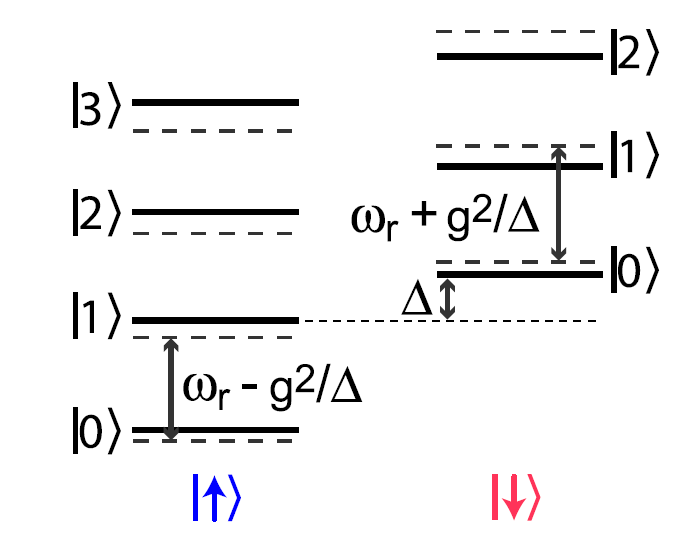
\includegraphics[width=0.5\linewidth]{pictures/JCenergy}
	\caption{Энергетическая структура системы cQED в дисперсионном режиме}
	\label{fig:jcenergy}
\end{figure}

Таким образом, частота резонансного отклика системы кубит+резонатор на внешнее возбуждение зависит от состояния кубита, как показано на Рисунке 13.
\begin{figure}[!h]
	\centering
	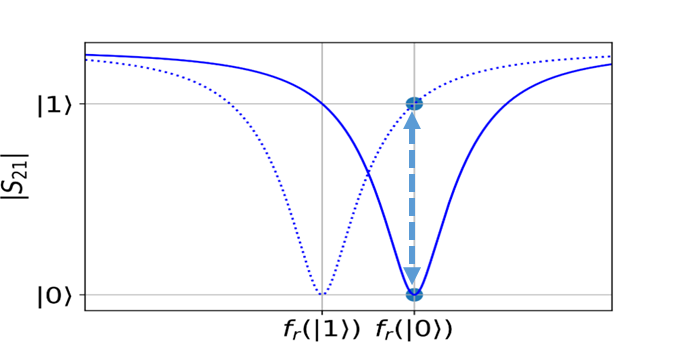
\includegraphics[width=0.5\linewidth]{pictures/dispshift}
	\caption{Дисперсионный сдвиг}
	\label{fig:dispshift}
\end{figure}
 
Зависимость частоты резонатора от состояния кубита лежит в основе дисперсионного считывания \cite{Chen2012} и двухтоновой спектроскопии \cite{Leng2011}. 

\subsection{Дисперсионное считывание. Квадратурные модуляция и демодуляция}
Для считывания квантовых состояний двухуровневых систем необходимо уметь генерировать короткие импульсы на частоте резонатора. Для этого  в работе использовались квадратурные смесители (IQ-Mixers). Это устройства, работающие по схеме, изображённой на Рисунке 14.

\begin{figure}[h]
	\centering
	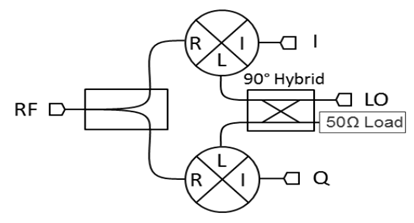
\includegraphics[width=0.5\linewidth]{pictures/IQ-mixer}
	\caption{Схема работы квадратурного смесителя}
	\label{fig:iq-mixer}
\end{figure}
На канал RF подётся гармонический сигнал. На каналы I и Q можно подавать сигналы любой необходимой формы. Сигнал на выходе LO, задаётся соотношением:
\begin{equation}
\tag{40}
U_{LO}(t) = I(t)\sin{\omega t}+ Q_(t)\cos{\omega t}
\end{equation}

Во-первых, подавая на каналы I и Q сигналы прямоугольной формы, можно получить короткие импульсы на обеих квадратурах, контролирующие состояние кубита, подобно тому, как это было описано в (\ref{cohdin}). 

Во-вторых, на канал LO можно принимать сигнал на выходе из образца, и с помощью каналов I и Q можно разделять его на составляющие соответствующие обеим квадратурам. Эти процессы называются модуляцией и демодуляцией сигнала соответственно.

Дисперсионное считывание представляет собой отправку одинаковых сигналов через образец на канал LO и напрямую из генератора на канал RF и его последующую демодуляцию. Результат такой демодуляции представлен на Рисунке 15:

\begin{figure}[!h]
	\centering
	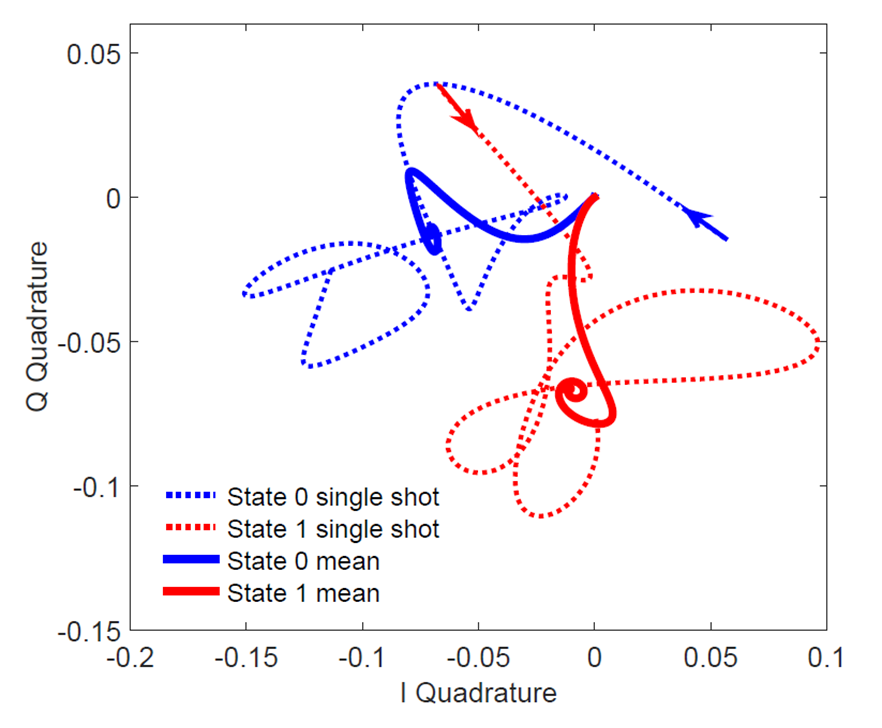
\includegraphics[width=0.5\linewidth]{pictures/readout}
	\caption{Временная развёртка сигнала в IQ-пространстве \cite{Magesan2015} }
	\label{fig:readout}
\end{figure}

По существу это измерение величины напряжение на каналах I и Q миксера в каждый момент времени. Очевидно, что вид таких "траекторий"  зависит резонансной частоты резонатора, а значит и от состояния кубита. 
   
	\clearpage
	\section{Основная часть}
\subsection{Экспериментальное оборудование. Схема экспериментальной установки}
\subsubsection{Криостат растворения}

Экспериментальная работа проводилась со сверхпроводящими квантовыми схемами, что подразумевает оперирование системой в условиях сверхнизких температур. Во-первых это даёт возможность обеспечить переход в сверхпроводящее состояние, во-вторых, и что более важно, в этом случае равновесная заселённость близка к чистому состоянию $|0\rangle$. Криостат растворения Oxford Instruments Triton DR-200, изображённый на Рисунке 16, стабильно обеспечивает температуру порядка 20 мК. 

\begin{figure}[h]
	\begin{minipage}[h]{0.49\linewidth}
		\center{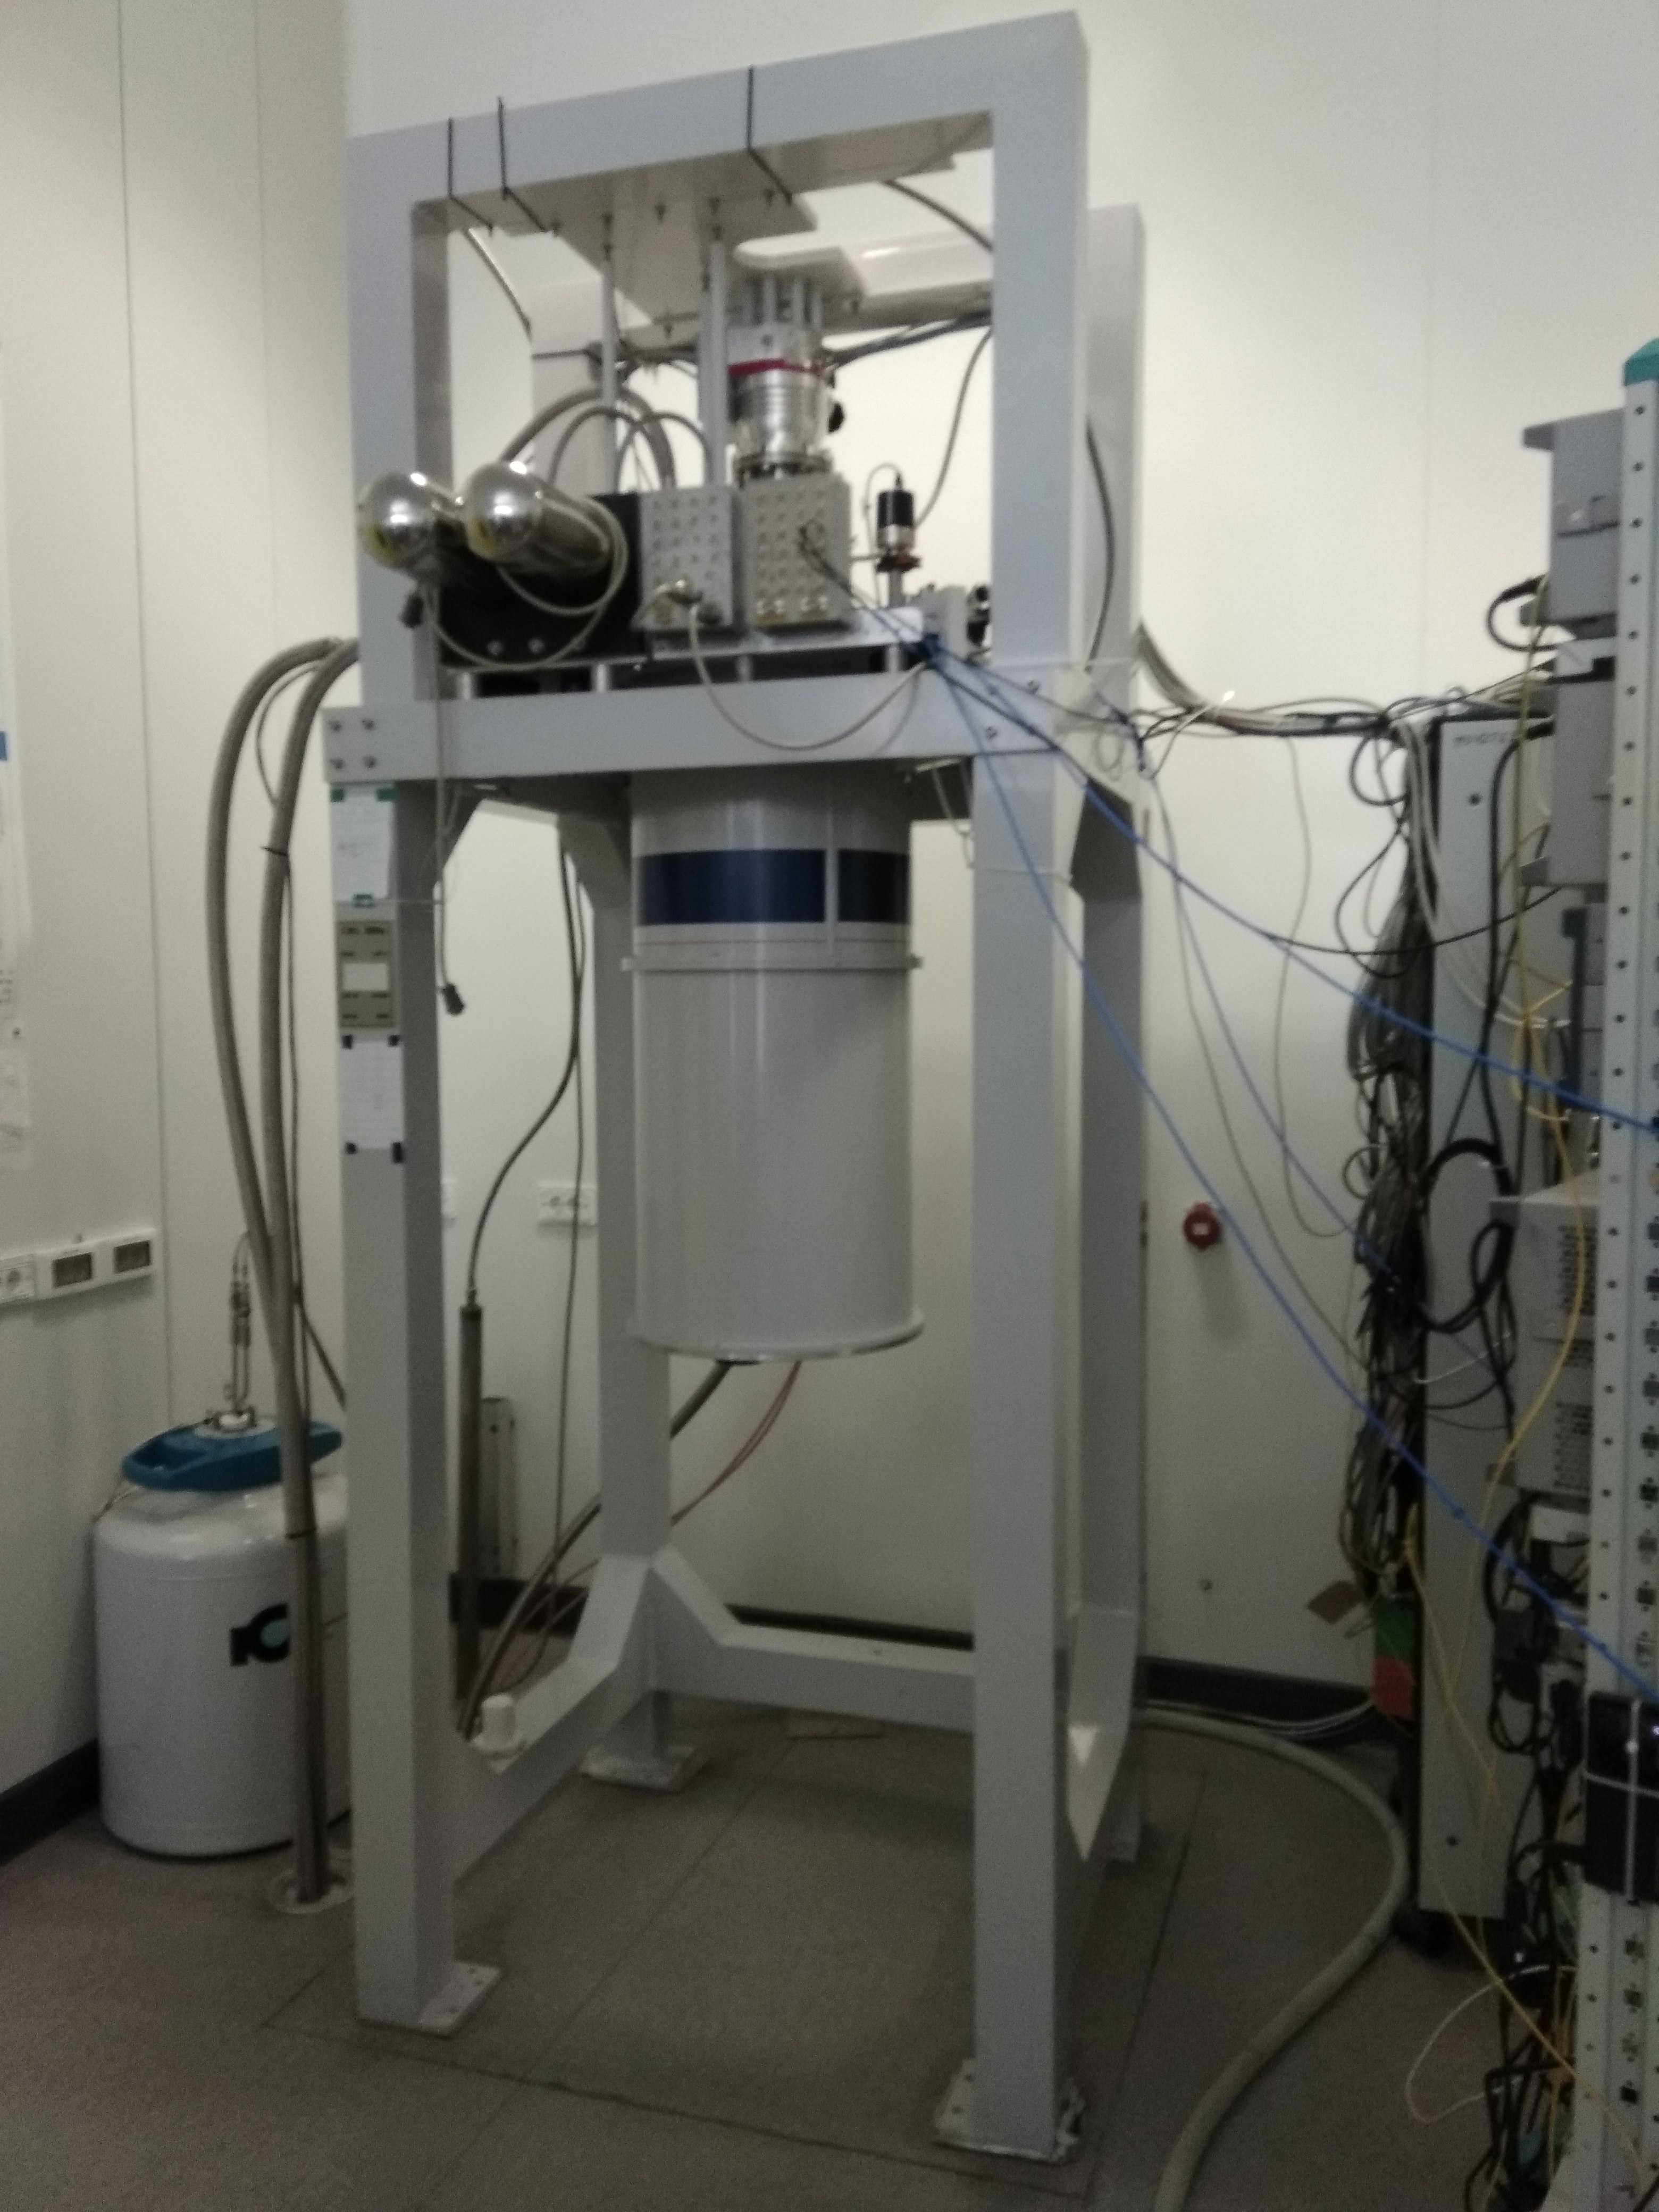
\includegraphics[width=0.9\linewidth]{pictures/IMG_20180614_120849} \\ а)}
	\end{minipage}
	\hfill
	\begin{minipage}[h]{0.49\linewidth}
		\center{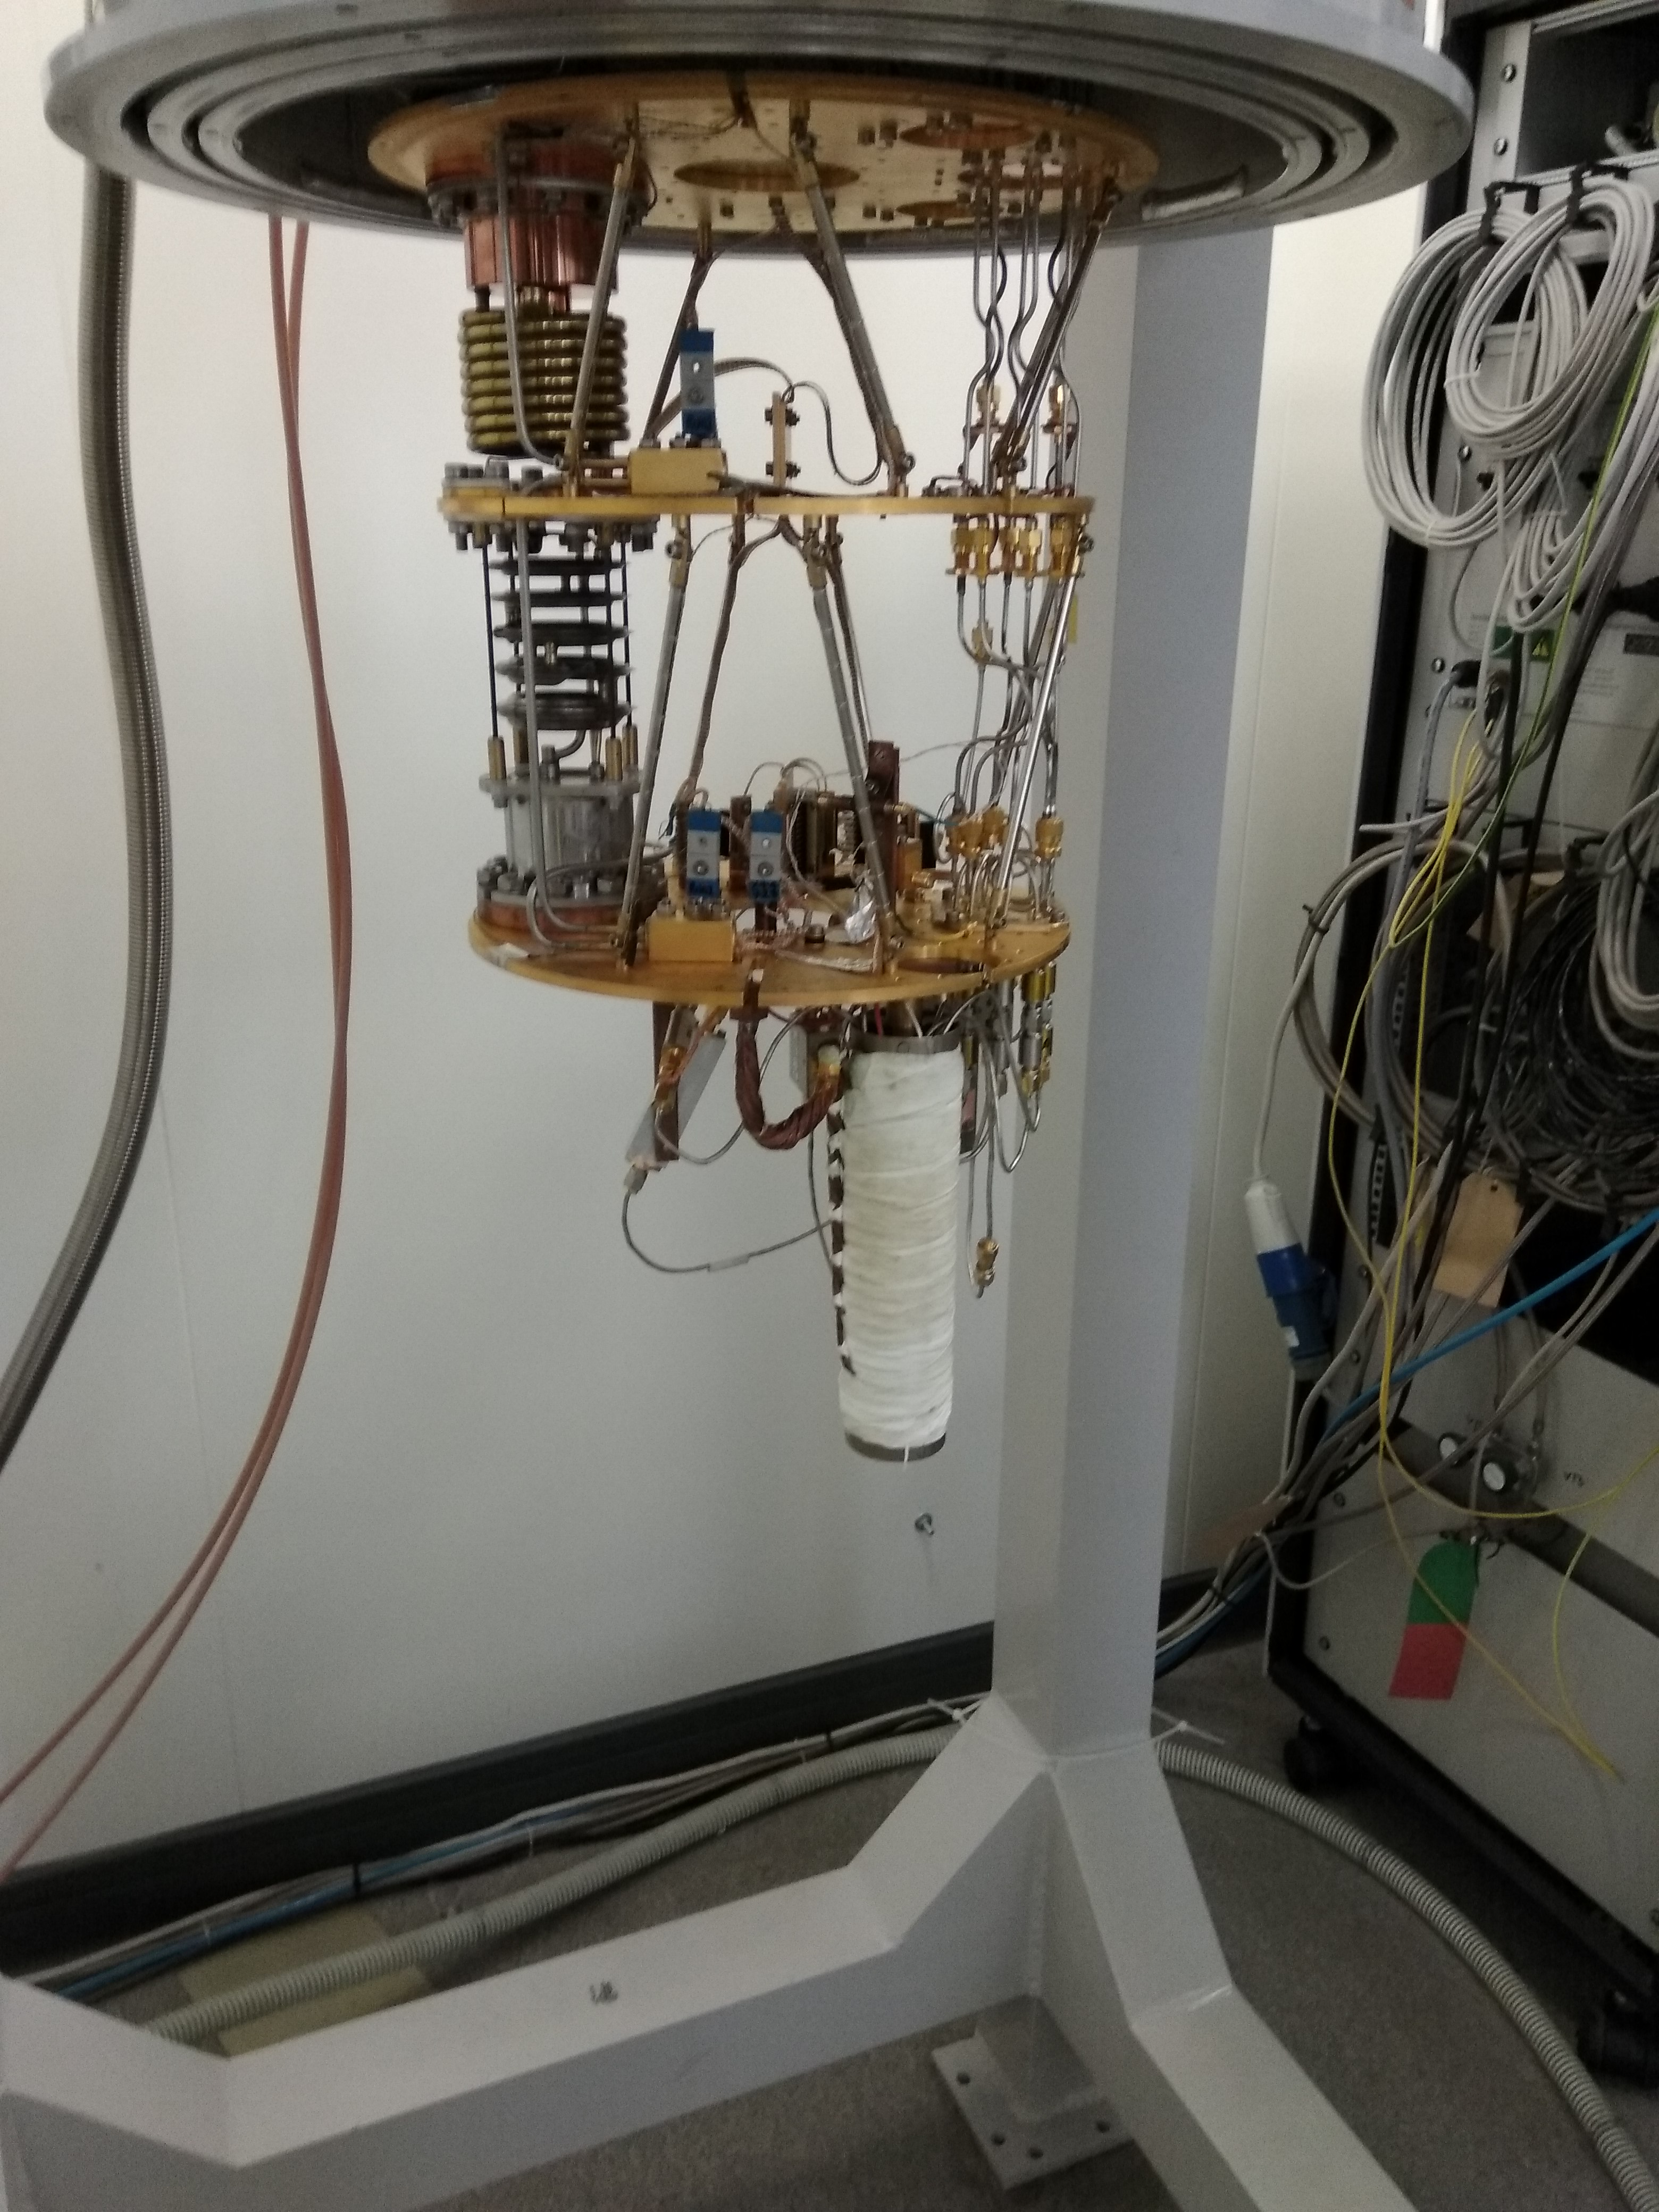
\includegraphics[width=0.9\linewidth]{pictures/IMG_20180614_123849} \\ б)}
	\end{minipage}
	\caption{Криостат растворения в закрытом (а) и открытом (б) видах}
	\label{ris:image1}
\end{figure}

Устройство состоит из турбомолекулярного насоса, для откачки паров ${^{3}He}$, компрессора для контроля криогенной системы, а так же вакуумной камеры, в которую и помещаются образцы. Вакуумная камера содержит несколько ступеней с последовательно усиливаемым охлаждением. Для минимизации теплообмена с окружающей система окружена экранами в виде концентрических цилиндров. Перед охлаждением систему откачивают до давления порядка $10^{-6}$ мбар. 

Т.к. воздействие на образец происходит посредством микроволновых сигналов, в криостат проведено 8 коаксиальных линий,а  так же медные провода для подачи постоянного тока.

В основе принципа работы лежит поглащение тепла при переходе фазы $^{3}He$ в $^{4}He$. На первом этапе происходит термо-акустическое охлаждение смеси  $^{3}He$ - $^{4}He$ до температуры порядка 700 мК. В силу того, что  $^{3}He$ легче, чем $^{4}He$ в результате этого процесса он оказывается сверху. Затем $^{3}He$ начинают откачивать, для того чтобы компенсировать потерю $^{3}He$ атомы вынуждены перемещаться в новые равновесные положения растворяясь при этом в смеси $^{3}He$ - $^{4}He$. Для того чтобы этот процесс происходил непрерывно в схему добавляется дополнительный импеданс для протекания процесса Джоуля - Томпсона для циркуляции смеси. Схема контура охлаждения представлена на Рисунке 17. 
\begin{figure}[h]
	\centering
	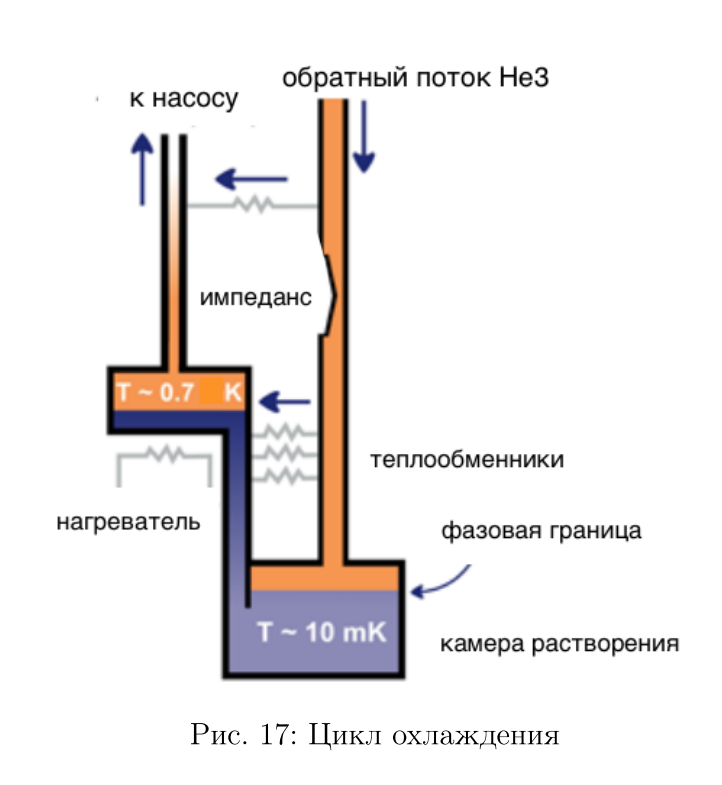
\includegraphics[width=0.5\linewidth]{pictures/fridgesheme}
	\caption{Схема контура охлаждения}
	\label{fig:fridgesheme}
\end{figure}
 
 \subsubsection {Аналого-цифровой преобразователь и ПЛИС}\label{adsfpga}
 Центральной частью данной работы было создание программного контроля для системы АЦП+ ПЛИС. АЦП (аналого-цифровой преобразователь) - устройство, преобразующее непрерывный аналоговый сигнал на входных каналах в дискретный цифровой. Для проведения экспериментов использовался 14-битный АЦП модели ADS54j40EVM компании Texas Instruments, частота дискретизации которого составляет 1000 сэмплов/сек. Модель представлена на Рисунке 18.
 
 \begin{figure}[!h]
 	\centering
 	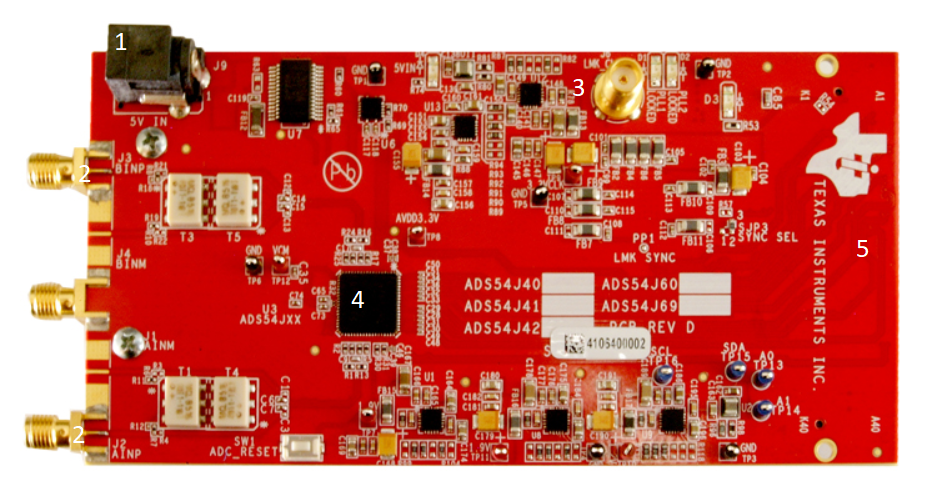
\includegraphics[width=0.7\linewidth]{pictures/ads}
 	\caption{ADS54j40EVM. Здесь 1 - канал питания, 2 - аналоговые входы, 3 - sma-разъём для синхронизирующего сигнала, 4 - чип с АЦП, 5 - разъём для связи с ПЛИС. Дополнительно на обратной стороны платы расположен тактовый генератор  }
 	\label{fig:ads}
 \end{figure}

ПЛИС (программируемая логическая интегральная схема) - полупроводниковое устройство, функционал которого генерируется пользователем уже после получения прибора. Программирование происходит путём изменения логики функционирования принципиальной схемы с помощью программирования на языке Verilog  и программного обеспечения Quartus Prime Software. Использование ПЛИС обусловлено значительно больше скоростью её работы по сравнению с обычными процессорами персональных компьютеров. Высокая скорость достигается в основном за счёт отсутствия ненужных в данной ситуации, интерфейсов, применяемых для общения с пользователем. Плата с ПЛИС TSW14J56EVM, использованной в работе, изображена на Рисунке 19.
\begin{figure}[h]
	\centering
	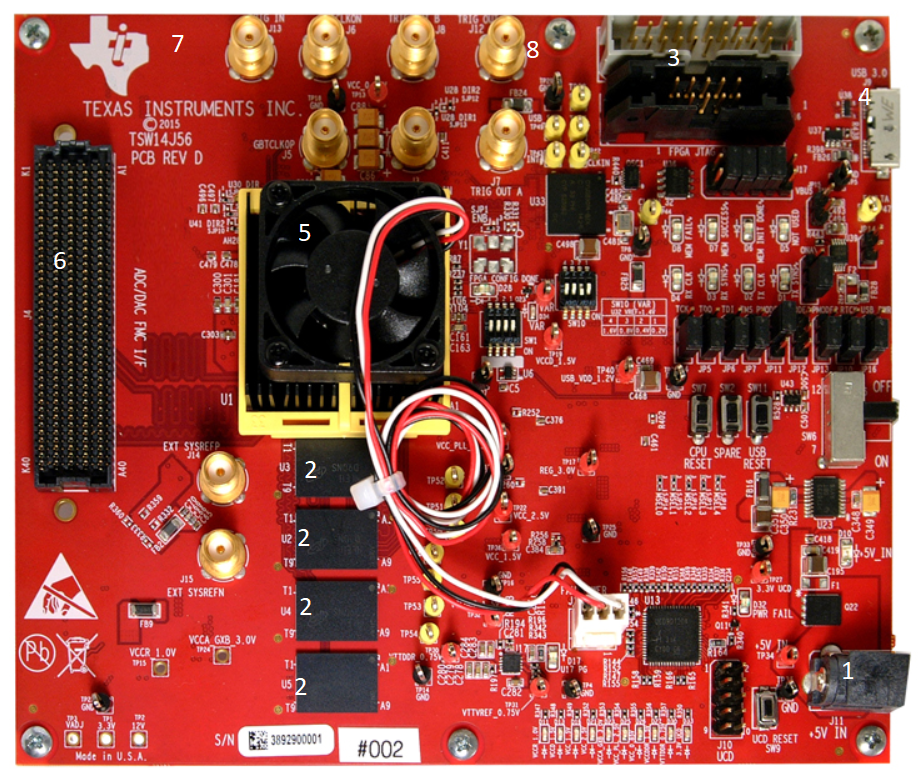
\includegraphics[width=0.5\linewidth]{pictures/fpga}
	\caption{ПЛИС TSW14J56EVM. Здесь 1 - канал питания, 2 - чипы с внешней памятью DDR, 3 - разъём JTAG для программирования ПЛИС, 4 - разъём USB для передачи данных с и на компьютер, 5 - чип с ПЛИС, 6 разъём для связи с АЦП, 7-8 каналы для получения и отправки триггеров во внешние устройства }
	\label{fig:fpga}
\end{figure}

Система ПЛИС+АЦП взаимодействует через JESD204b. Это интерфейс синхронной последовательной передачи больших объёмов данных. Суть его сводится к конвертации оцифрованного сигнала, представляющего собой значения на каждом из 14 бит каждого из двух каналов  АЦП в форму удобную для последующей обработке на ПЛИС а так же непосредственной передаче в виде последовательности 256-битных сегментов. 

На выходе JESD204b соединён со следующим виртуальным модулем, суть которого сводится к синхронному захвату данных из JESD, конвертации их в 256 бит в 512 и записи 512-битных сегментов в во внешнюю память. Следующая ступень, считывание из памяти и отправка данных по USB на ПК через интерфейс GPIF II. Синхронизация ПЛИС и АЦП обеспечивается интерфейсом JESD204b, а синхронизация АЦП и ПЛИС с внешними генераторами сигналов производится с помощью триггеров приходящих на аналоговые sma-разъёмы устройств.

\subsubsection{Схема экспериментальной установки}  
Помимо оцифровки сигнала и поддержания низких температур перед экспериментатором ставится ещё целый ряд задач, связанных в основном с генерированием сигналов правильной формы для считывания и контроля состояний кубитов. Для этих целей используются приборы, изображённый на Рисунке 20:

\begin{figure}[h]
	\centering
	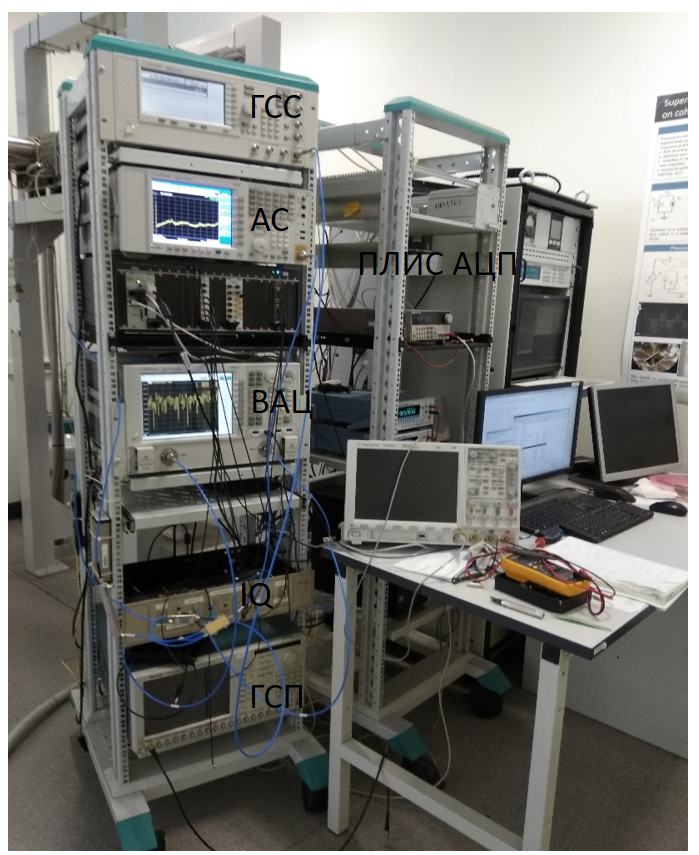
\includegraphics[width=0.6\linewidth]{pictures/shema1}
	\caption{Микроволновое оборудование}
	\label{fig:shema1}
\end{figure}


Всё это оборудование соединяется в специальную схему, дающую возможность генерировать как импульсный сигнал, для контроля и считывания состояний, так и непрерывный для проведения спектроскопии образцов. Здесь есть генератор высокочастотного синусоидального сигнала, анализатор спектров, векторный анализатор цепей, квадратурные смесители, генератор сигналов произвольной формы, осциллограф и АЦП+ПЛИС система. Всё это соединено по схеме, представленной на Рисунке 21. 

\begin{figure}[t!]
	\centering
	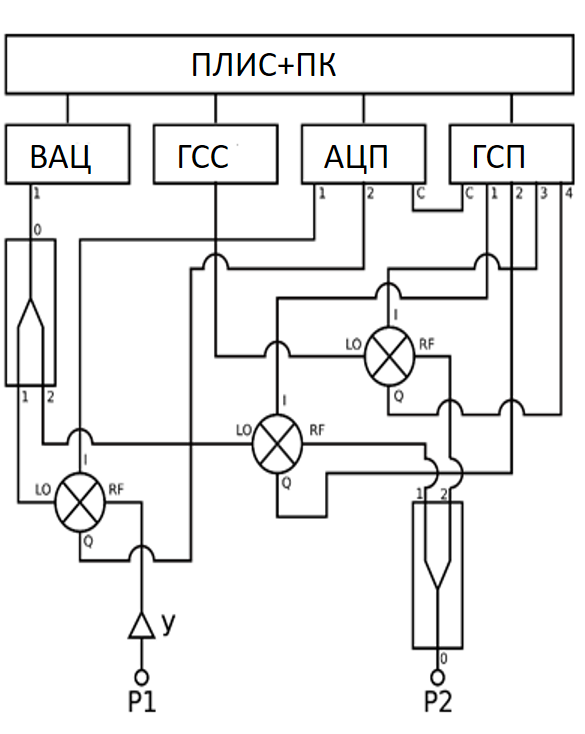
\includegraphics[width=0.5\linewidth]{pictures/shema}
	\caption{Схема соединения экспериментального оборудования}
	\label{fig:shema}
\end{figure}

\subsection{Спектроскопия образцов}
\subsubsection{Однотоновая спектроскопия}\label{sigletone}
Очевидно, что для манипуляции и считывания кубитных состояний нужно знать, на какой частоте подавать сигналы. Поэтому любые измерения начинаются с поиска спектров резонатора и кубитов. Как было сказано в (\ref{transmon}) используя СКВИД можно перестраивать частоту перехода кубита в зависимости от внешнего магнитного потока. Частота резонатора при этом не меняется. Для проведения однотоновой спектроскопии  последовательно подаётся сигнал на разных частотах и меняется внешний магнитный поток с использованием постоянного тока. В результате получается зависимость коэффициента прохождения на ВАЦ от внешнего потока и частоты сигнала, как изображено на Рисунке 22. 

Частота кубита косинусоидально зависит от внешнего потока, поэтому на Рисунке 22 видно пересечение прямой линии, отвечающей резонатору с косинусоидальной, отвечающей кубиту. В точках пересечения наблюдается вырождение состояний отвечающих нахождению фотона в кубите и в резонаторе. 

\begin{figure}[t]
	\centering
	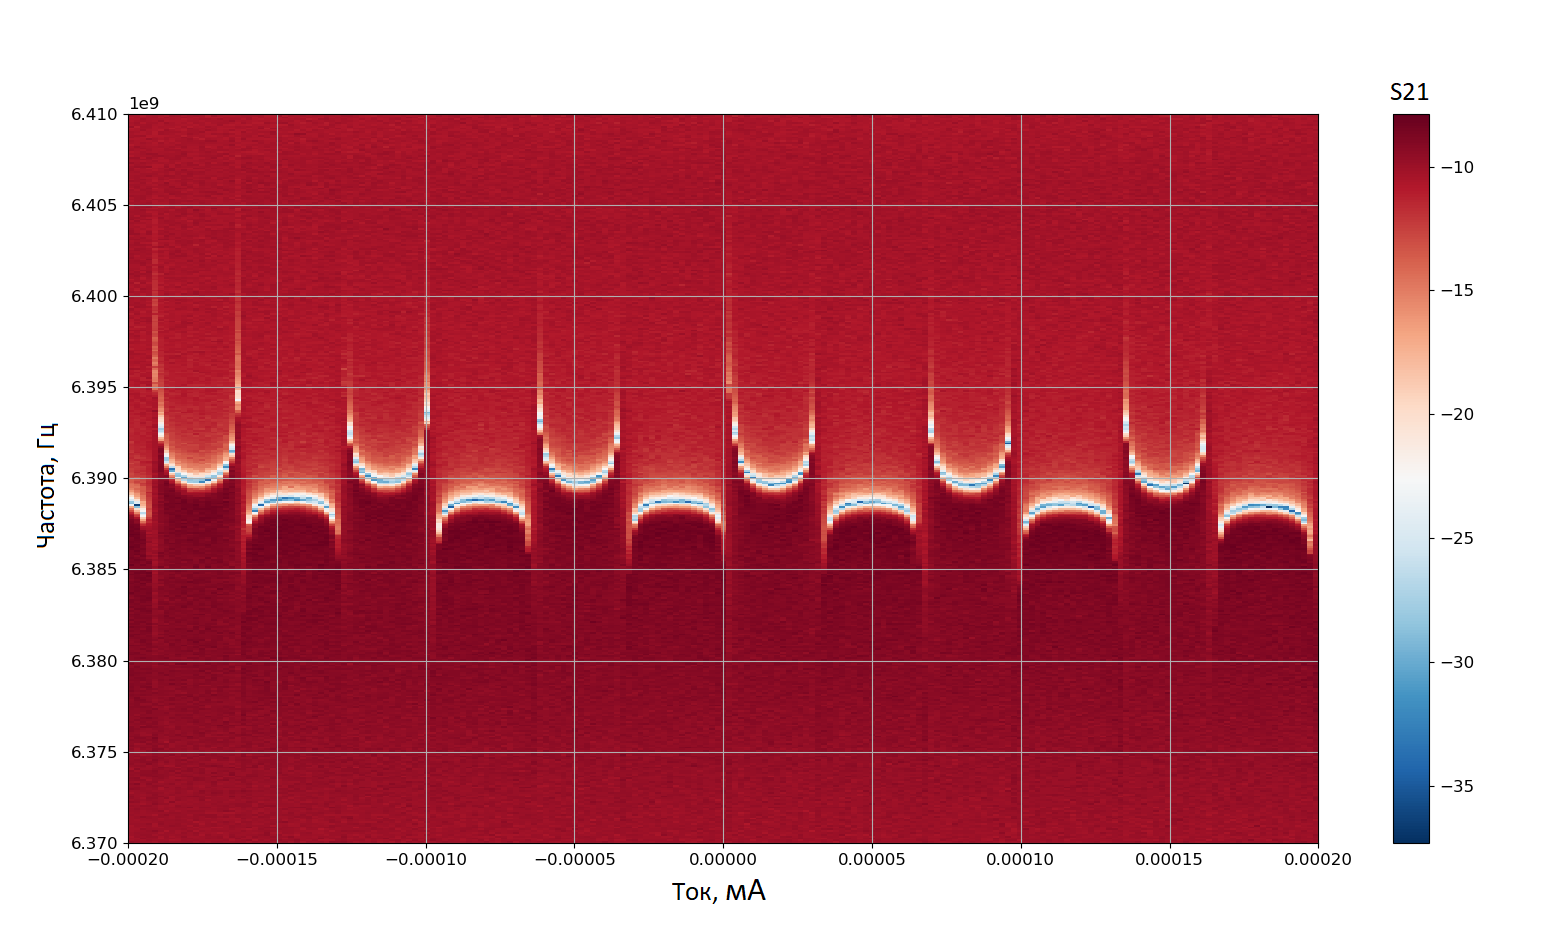
\includegraphics[width=0.9\linewidth]{pictures/anticross_6_39}
	\caption{Однотоновая спектроскопия}
	\label{fig:anticross639}
\end{figure}

Точки вырождения на однотоновом спектре обычно называют антикроссингами или квазипересечениями. Они дают информацию о том, при каком токе стоит искать минимум и максимум частоты кубита. Стоит заметить, что все воздействия на перестраиваемые кубиты происходят или в максимуме или в минимуме частоты, потому что там кубит менее восприимчив к потоковым шумам. 

\subsubsection{Двухтоновая спектроскопия}
Определившись со значениями частоты резонатора и тока для максимальных и минимальных частот кубита, можно переходить к двухтоновой спектроскопии. Результат измерения представлен на Рисунке 22: 
\begin{figure}[!h]
	\centering
	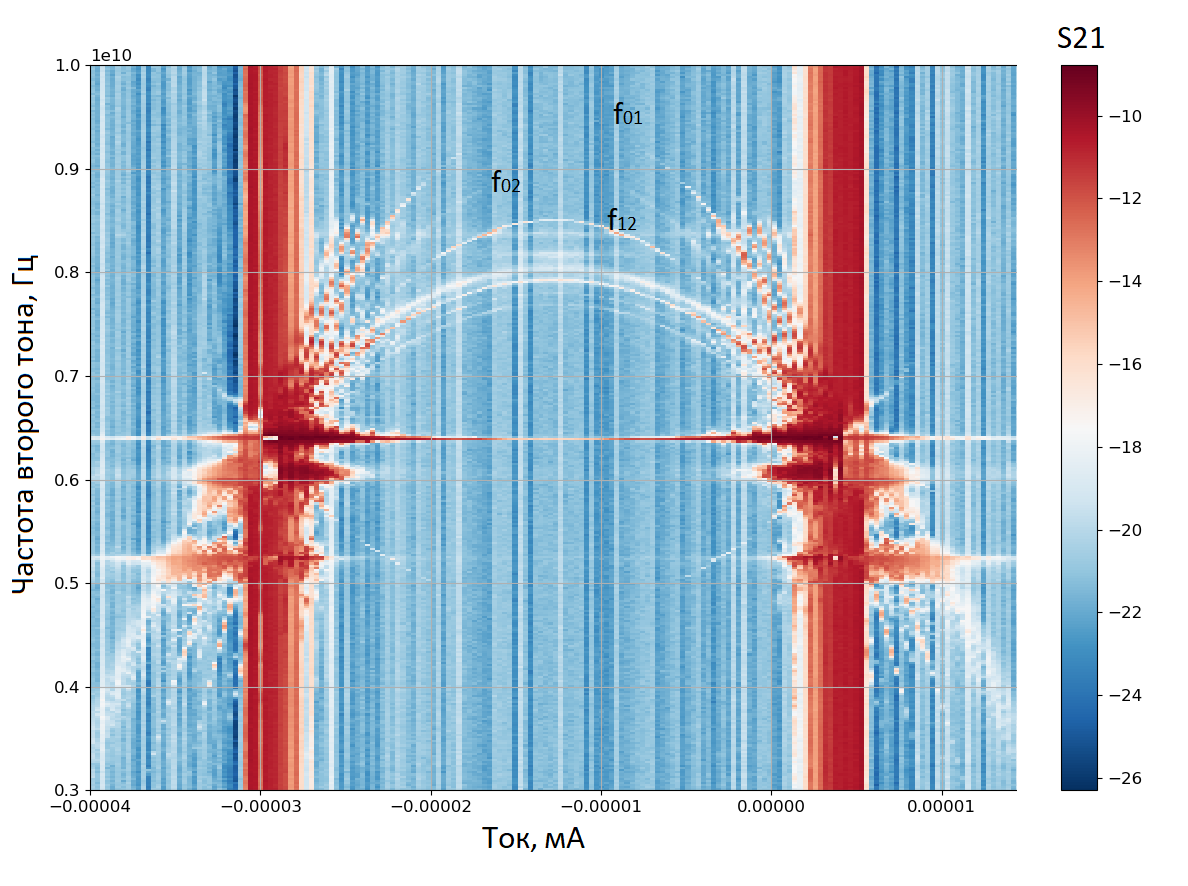
\includegraphics[width=0.8\linewidth]{pictures/2tone6_39}
	\caption{Двухтоновый спектр}
	\label{fig:2tone639}
\end{figure}

Принцип её работы основан на эффекте описанном в (\ref{transres}), В отличие от однотоновой спектроскопии здесь присутствует два сигнала. Один генерируется на частоте, равной частоте резонатора, найденной в (\ref{sigletone}), второй в некотором диапазоне частот, в которую, предположительно входит максимальная частота кубита. Перестраивая частоту кубита постоянным, можно наблюдать косинусоидальную линию, соответствующую кубиту, и прямую линию соотвествующую резонатору. Стоит заметить, что спектроскопия проводилась при большой мощности кубитного тона и потому на спектре видно сразу несколько переходов в трансмоне. 

\subsection{Импульсные измерения}
\subsubsection{Осцилляции Раби}

Импульсные измерения кубитов начинаются с наблюдений осцилляций Раби, подобно тому, как это было описано в (\ref{cohdin}). Для этого с помощью квадратурных смесителей и генератора сигналов произвольной формы из непрерывного синусоидального сигнала вырезаются прямоугольные импульсы и отправляются на образец. Затем посылается считывающий сигнал. Последовательность импульсов изображена на Рисунке 23.
\begin{figure}[h]
	\centering
	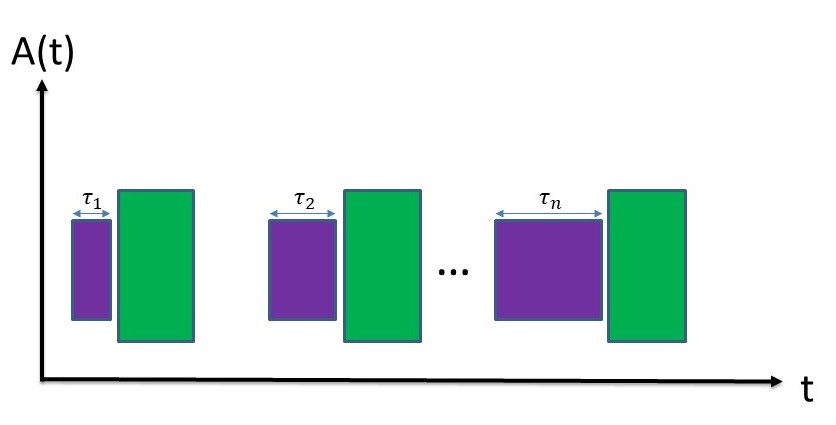
\includegraphics[width=0.6\linewidth]{pictures/Rabipulseseq}
	\caption{Последовательность импульсов для наблюдения осцилляций Раби. Зелёным цветом изображён импульс на частоте резонатора, а фиолетовым на частоте кубита}
	\label{fig:rabipulseseq}
\end{figure}

Как видно из Рисунка 23,  длительность возбуждающего кубит импульса $\tau_i$ меняется в некотором диапазоне значений. В результате такой последовательности наблюдается картина изображённая на Рисунке 24. Данные аппроксимируются функцией вида $e^{-\frac{t}{t}} \sin{\omega_r t}$, где $\omega_r$ это частота Раби-осцилляций. Знание Раби-частоты даёт информацию о длительности сигнала, необходимого для перевода кубита из одного состояния в другое. 

Так например время $\pi$- импульса, т.е. импульса под действием которого квантовое состояние совершает поворот на $180^{\circ}$, составляет половину Раби-периода.
\clearpage

\begin{figure}[h]
	\centering
	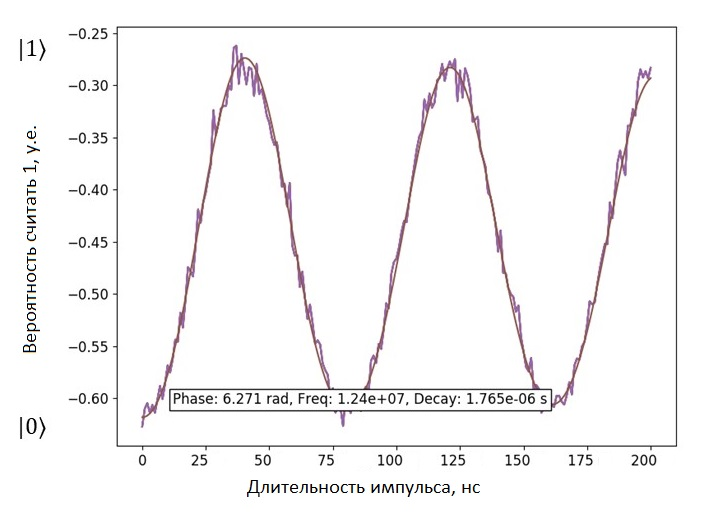
\includegraphics[width=0.7\linewidth]{pictures/rabires.png}
	\caption{Раби осцилляции. Фиолетовым цветом - экспериментальные данные, коричневым - подгоночная кривая}
	\label{fig:rabires}
\end{figure}


\subsubsection{Время когерентности и релаксации}
Как было показано в  (\ref{neun}) взаимодействие с окружением разрушает чистое квантовое состояние, переводя его в смешанное. Для того чтобы обладать информацией о длительности того промежутка времени, в течение которого кубит пригоден для проведения квантовых алгоритмов измеряются два характерных параметра.

Первый параметр - время когерентности, т.е. время, за которое квантовое состояние становится из максимально чистого максимально смешанным под действием дефазировки. Эксперимент по измерению этого времени называется наблюдением осцилляций Рамзи. Импульсная последовательность для этого случая изображена на Рисунке 26:

\begin{figure}[h]
	\centering
	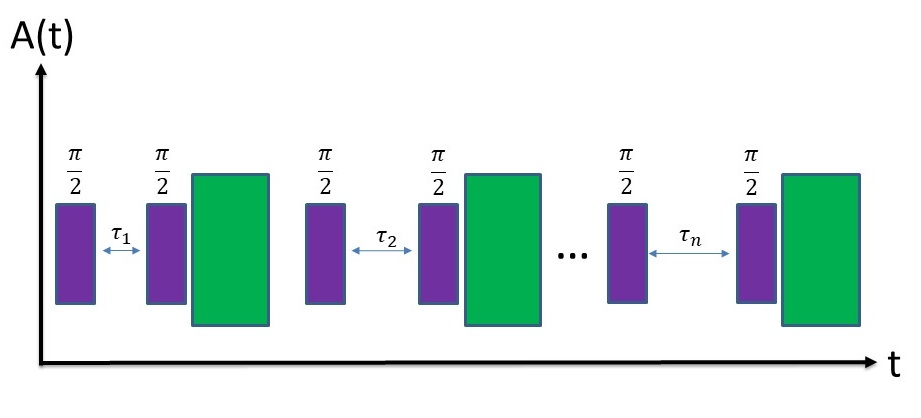
\includegraphics[width=0.6\linewidth]{pictures/Ramseypulseseq}
	\caption{Последовательность импульсов при наблюдении осцилляций Рамзи}
	\label{fig:ramseypulseseq}
\end{figure}

 Суть её заключается в следующем. На кубит подётся $\frac{\pi}{2}$ - импульс, который переводит квантовое состояние на экватор сферы Блоха. Там, как было показано в (\ref{neun}) ввиду наличия дефазировки состояние начинает свободную прецессию вдоль экватора. После задержки $\tau$, величина которой варьируется от нуля до некоторого параметра, подаётся второй $\frac{\pi}{2}$. Естественно, если задержки между импульсами не было, то два $\frac{\pi}{2}$ импульса эквивалентны одному $\pi$, в таком случае кубит окажется в состоянии $|1\rangle$. Но если вектор состояния прошёл половину экватора сферы Блоха, переместившись, к примеру, из состояния $|+\rangle$ в состояние $|-\rangle$, второй $\frac{\pi}{2}$-импульс переведёт его обратно в состояние $|0\rangle$. Итоговый график изображён на Рисунке 27:
 
 \begin{figure}[h]
 	\centering
 	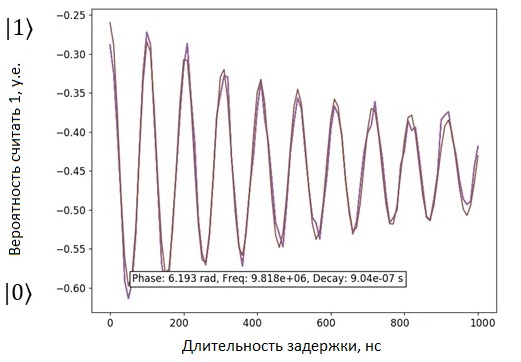
\includegraphics[width=0.7\linewidth]{pictures/ramseyres.png}
 	\caption{Осцилляции Рамзи. Фиолетовый цвет - экспериментальные данные, коричневый - подгоночная кривая}
 	\label{fig:ramseyres}
 \end{figure}

Результат аппроксимируется функцией вида $e^{-\frac{t}{T_2}}\sin{\omega t}$, здесь $T_2$ - время когерентности кубита,т.е. время, за которое вероятность считать $|1\rangle$ после второго $\frac{\pi}{2}$-импульса уменьшилась в e раз, а частота этих осцилляций равна отстройке частоты сигнала от частоты кубита. Используя этот параметр, можно точнее подбирать частоту сигнала для контроля квантового состояния. 

Второй параметр - время релаксации $T_1$. Физическая величина, отражающая скорость распада перехода кубита из чистого состояния $|1\rangle$ в смешанное состояние равновесия. Импульсная последовательность представлена на Рисунке 28.

\begin{figure}[h]
	\centering
	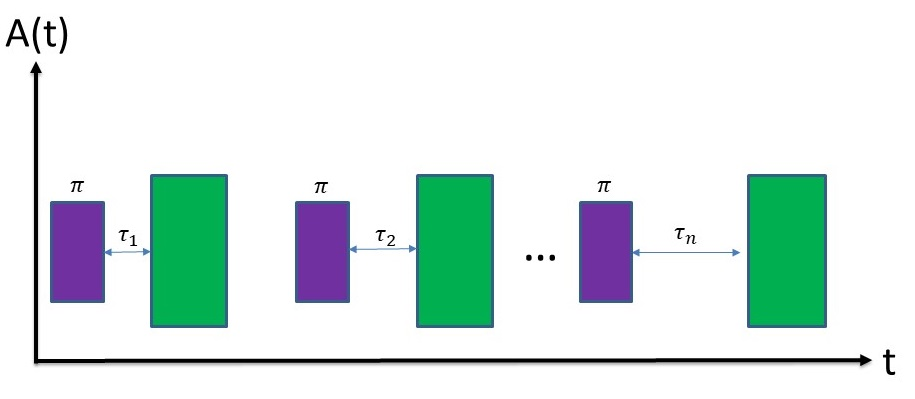
\includegraphics[width=0.6\linewidth]{pictures/todinpulseseq}
	\caption{Последовательность импульсов для определения времени релаксации}
	\label{fig:todinpulseseq}
\end{figure}

В этом эксперименте необходимо перевести кубит в состояние $|1\rangle$ и через некоторый промежуток времени послать считывающий импульс. Производится скан по величине промежутка. Результат представлен на Рисунке 29.

\begin{figure}[h]
	\centering
	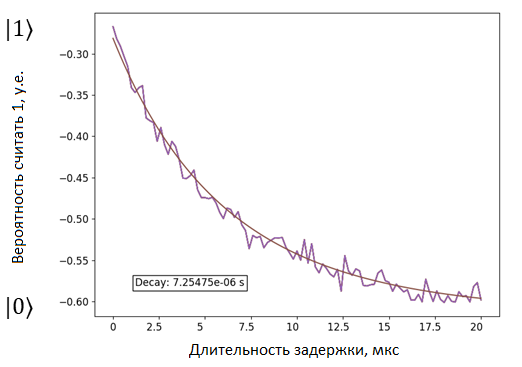
\includegraphics[width=0.7\linewidth]{pictures/t1res.png}
	\caption{Релаксация квантового состояния.Фиолетовым цветом - экспериментальные точки, коричневым подгоночная кривая}
	\label{fig:t1res}
\end{figure}

В этот раз данные фитуются затухающей экспонентой, а время релаксации - величина обратная декременту затухания. 

\subsection {Дискриминация квантовых состояний}\label{discr}
Одной из задач машинного обучения является так называемая задача статистической классификации. Она состоит в присваивании произвольной выборке значений определённого класса в зависимости от статистических характеристик данной выборки. Компьютерные алгоритмы решения такого рода задач широко используются в медицине, геолого-разведочных операция и целом ряде других задач. Не является исключением и экспериментальная квантовая информатика, в которой задача классификации используется при считывании.

После определения частот и длительностей возбуждающих и считывающих сигналов, а так же характерных времён, в течение которых возможно оперирование квантовой системой можно приступить к ряду новых задач. Одной из таких задач является единовременное считывание квантового состояния (Single shot readout).  

Концепция такого считывания состоит в следующем. На кубит посылается считывающий импульс. Как всегда по кабелям он доходит до чипа, проходит по передающей линии или уходит в резонатор в зависимости от состояния кубита. Так или иначе, на выходе из криостат результат приходит на АЦП. Как было указано ранее (\ref{adsfpga}) такой результат представляет собой развёртку значений напряжений во времени. И внешний вид напряжения, как функции времени напрямую зависит от состояния кубита. Пример такой зависимости представлен на Рисунке 30.


\begin{figure}[h]
	\centering
	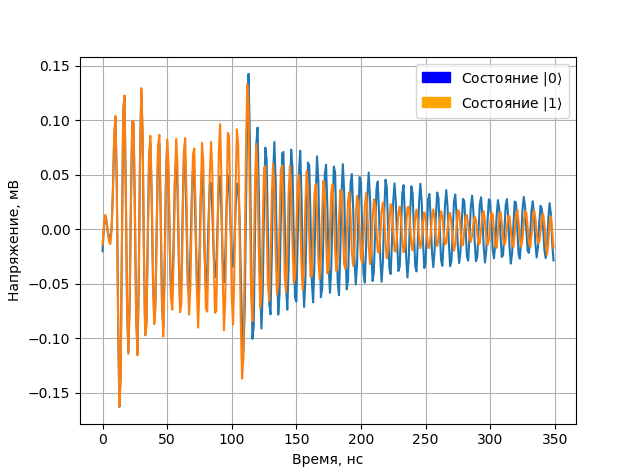
\includegraphics[width=0.7\linewidth]{pictures/Etalones}
	\caption{Вид считывающих импульсов соответствующих разным квантовым состояниям}
	\label{fig:etalones}
\end{figure}

С точки зрения задачи классификации каждый такой считывающий импульс представляет собой некоторую статистическую выборку. И каждому из них необходимо присвоить класс, (в данном случае класс $|0\rangle$ и $|1\rangle$) и, следовательно считать состояние. 

В работе использовалось два классификатора. Первым из них был линейный дискриминатор (LDA). Процесс обучения состоял из ряда этапов. С заранее известным состоянием производится 50000 повторений записи значений напряжения для каждого из классов. Далее случайные $70 \%$ от общего числа записей отделяются. Для них считается среднее напряжение как функция времени:

\begin{equation}
\tag{41}
\mu(t) = \frac{1}{n}\sum_{n=1}^{35000} V_n(t)
\\
\end{equation}

На этом процесс обучения линейного дискриминатора заканчивается и начинается процесс тестирования. Для каждой из оставшихся выборок считается разность коэффициентов ковариации с $\mu_0(t)$ и $\mu_1(t)$.

\begin{equation}
\tag{42}
K_n = \langle V_n\rangle\langle\mu_0(t)\rangle - \langle V_n\rangle\langle\mu_1(t)\rangle
\\
\end{equation}

При этом если величина $K_n$ положительна, состояние классифицируется, как $|0\rangle$, а если отрицательна - как $|1\rangle$. 

Вторым классификатором был квадратичный (QDA). В этом случае на тренировочной выборке помимо среднего значения считается так же ковариационная матрица:
\begin{equation}
\tag{43}
\Sigma_{ij} = cov(X_i,X_j)
\end{equation}

Здесь $X_i$- вектор размерности выборки. Т.е. по существу, это матрица, которая показывает, величину дисперсии определения значения в каждой точке по времени.

В случае QDA формула классификации имеет вид:
\begin{equation}
\tag{45}
Q_n = -\frac{1}{2}V^T(\Sigma_0^{-1}- \Sigma_1^{-1})V+ V^T(\Sigma_0^{-1}\mu_0- \Sigma_1^{-1}\mu_1)
\end{equation}
А величина порога, которая для LDA являлась нулём, считается из соотношения:
\begin{equation}
\tag{46}
Q_{tresh}= \frac{1}{2}(\mu_0^T\Sigma_0^{-1}\mu_0 - \mu_1^T\Sigma_1^{-1}\mu_1)+\frac{1}{2}\log{\frac{|\Sigma_0|}{|\Sigma_1|}}
\end{equation}
Здесь $|\Sigma_i|$ - определители матриц. 

Соотвественно, если величина $Q_n$ больше, чем $Q_{tresh}$, то состояние классифицируется как $|0\rangle$, в противном случае как $|1\rangle$.Критерием считывания в простейшем случае является величина фиделити, определяемая из формулы:
\begin{equation}
\tag{47}
F = 1 -\frac{N_{FP}+N_{FN}}{2},
\end{equation}
\noindent где $N_{FP}$ и $N_{FN}$ число неправильно определённых состояний $|0\rangle$  и $|1\rangle$ соотвественно. Фиделити линейного дискриминатора оказалось 75 \%, а фиделити QDA о 83 \%.

Результирующая гистограмма представлена на Рисунке 31:

\begin{figure}[h]
	\centering
	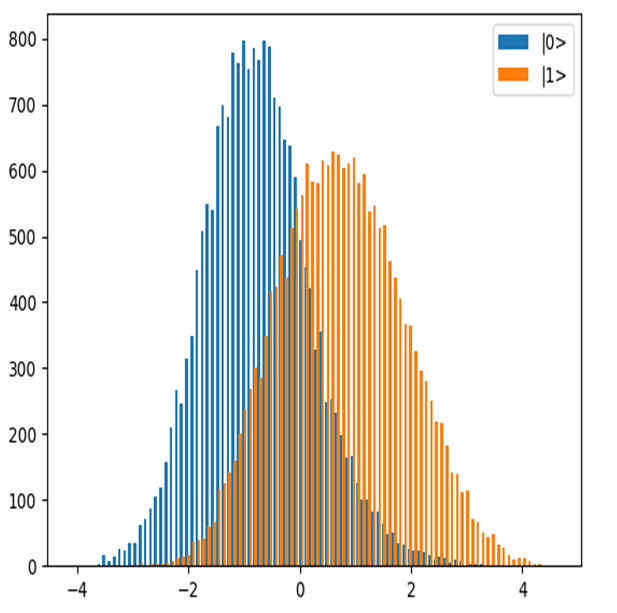
\includegraphics[width=0.5\linewidth]{pictures/resulthist}
	\caption{Гистограмма квантовых состояний $|0\rangle$ и $|1\rangle$}
	\label{fig:resulthist}
\end{figure}
\clearpage
\subsection{Двойное считывание}\label{doubleread}
С точки зрения считывания остался ещё один вопрос, на который пока не было дано ответа. В случае ошибки дискриминации, как понять, развалилось ли состояние до считывания или произошла ошибка классификации из-за наложившихся на сигнал шумов. Ответ на этот вопрос поможет найти двойное считывание.

Схема его состоит в следующем. На кубит в исходном состоянии $|0\rangle$ подаётся два считывающих импульса с варьируемой задержкой. Затем считается коэффициент их ковариации друг с другом, как функция задержки. Результат изображён на Рисунке 32:

\begin{figure}[h]
	\centering
	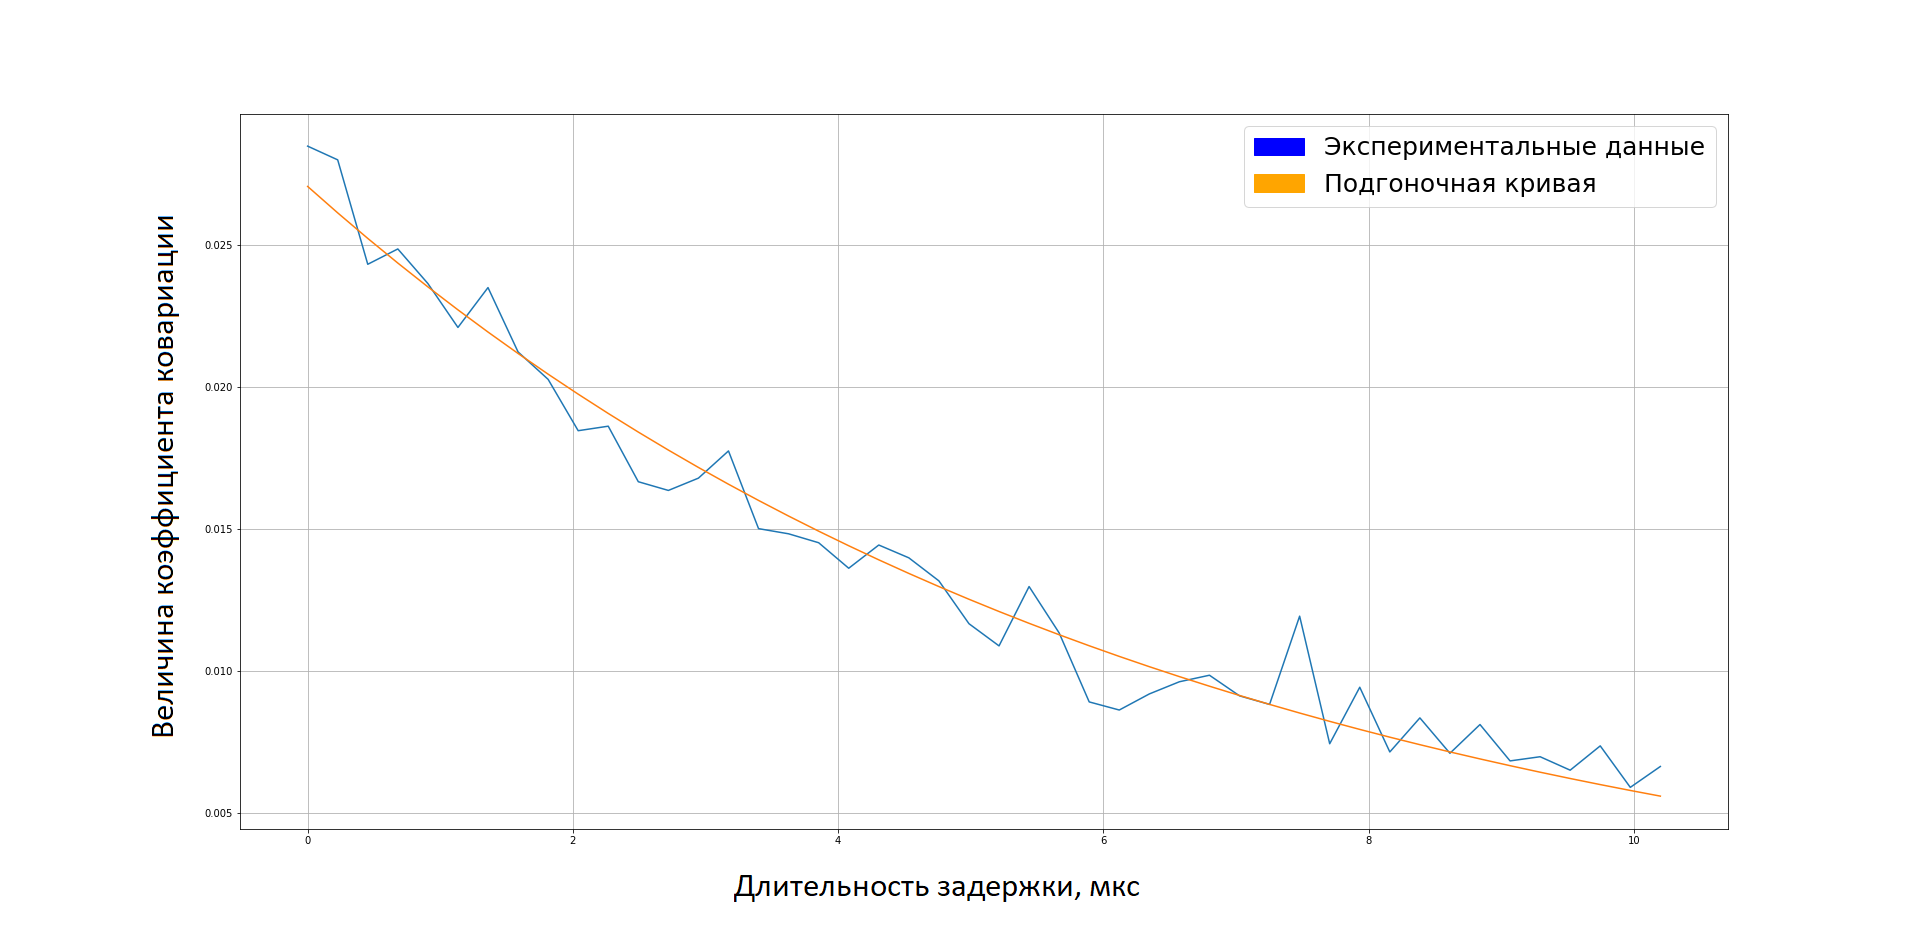
\includegraphics[width=0.8\linewidth]{pictures/result}
	\caption{Ковариация последовательных считывающих импульсов }
	\label{fig:result}
\end{figure}

Из этого графика можно получить три важных параметра, значение ковариации в первый момент времени, когда между импульсами не было задержки,декремент экспоненциального затухания и среднее значение состояния.

Далее составляется модель ошибок. Если считать, что существует только два типа ошибок – ошибка приготовления состояния (в дальнейшем $P_0$) и ошибка считывания ($P_r$). Первая ошибка – по причинам взаимодействия с тепловым окружением кубит изначально оказался в состоянии $|1\rangle$. Вторая ошибка – несмотря на то, что на самом деле кубит был в состоянии $|0\rangle$ в процессе обработки шумного сигнала он был классифицирован, как $|1\rangle$. В этом случае вероятности считать $|0\rangle$ и $|1\rangle$ в первом измерении вычисляются по формулам:
\begin{equation}
\tag{48}
\begin{split}
&P(Q_1 = 0)= 1- P_0 - P_r +P_0P_r\\
&P(Q_1 = 1)= P_0+P_r - P_0P_r
\end{split}
\end{equation}

Теперь надо подумать, что будет происходить с вероятностями двойного считывания. Во-первых, вероятность второй раз считать кубит в $|1\rangle$  если и первый раз он был в $|1\rangle$ должна в начальный момент времени быть равна 1-$P_r$ т.к. считать не единицу можно только  в случае ошибки считывания. А на больших временах, вероятность считать единицу складывается из вероятности ошибки считывания (из-за процессов некогерентной релаксации), ошибки приготовления (прошло какое-то время, в течение которого кубит находился в тепловом равновесии с окружением), за вычетом их произведения (так как, совершив обе ошибки,результат не изменится).

\begin{equation}
\tag{49}
\begin{split}
P(Q_2 = 1 | Q_1 = 1) &= e^{-\gamma t}(1-P_0 - P_r +P_0P_r-P_r)+ P_r +P_0-P_0P_r = \\
&e^{-\gamma t}(1-P_{relax}-P_r)+P_{relax},
\end{split}
\end{equation}
\noindent где $P_{relax} = P_r +P_0-P_0P_r$, а $\gamma$ коэффициент затухания ковариации последовательных считывающих импульсов.Соответственно, вероятность считать состояние $|0\rangle$ сразу после $|1\rangle$ выражается формулой:

\begin{equation}
\label{ubi}
\tag{50}
P(Q_2 = 0 | Q_1 = 1)= 1- e^{-\gamma t}(1-P_{relax}-P_r)+P_{relax}
\end{equation}

Чтобы найти вероятность состояния $|1\rangle$ при втором считывании, если результатом первого был $|0\rangle$ ,в  выражении (\ref{ubi}) $P_{relax}$ заменяется на $1-P_{relax}$:

\begin{equation}
\tag{51}
P(Q_2 = 1 | Q_1 = 0)= P_{relax} - e^{-\gamma t}(P_{relax}-P_r)+P_{relax}
\end{equation}

А для вероятности считать $|0\rangle$  второй раз,при первом исходе-$|0\rangle$:

\begin{equation}
\tag{51}
P(Q_2 = 0 | Q_1 = 0)= 1 - P_{relax} + e^{-\gamma t}(P_{relax}-P_r)
\end{equation}

 Для математического описания полученной экспериментальной зависимости и для извлечения из неё искомых вероятностей ошибок необходимо посчитать ковариацию этих двух считываний ($Q_1$  и $Q_2$ ):
 
 \begin{equation}
 \label{cov}
 \tag{52}
 Cov_{Q_1Q_2} = \langle Q_1 Q_2 \rangle - \langle Q_1\rangle\langle Q_2\rangle
 \end{equation}
 
Где $\langle Q_1 Q_2 \rangle = P_{relax}(e^{-\gamma t}(1-P_{relax}-P_r)+P_{relax})$ это среднее значение произведения результатов считываний, посчитанное, как произведение $P(Q_1 = 1) P(Q_2 = 1|Q_1 = 1)$. Значение $\langle Q_1 \rangle = P_{relax}$, а $\langle Q_2 \rangle$:
\begin{equation}
\tag{53}
\langle Q_2 \rangle = P(Q_1 = 1| Q_2 =1) + P(Q_1 = 1| Q_2 = 0)=
P_{relax}+P_re^{-\gamma t}-2P_{relax}P_re^{-\gamma t}
\end{equation}
Наконец, подстановка в (\ref{cov}) даёт следующий результат:
\begin{equation}
\tag{54}
Cov_{Q_1Q_2}= P_{relax}e^{-\gamma t}-P_{relax}^2e^{-\gamma t}+2P_rP_{relax}^2e^{-\gamma t}- 2P_re^{-\gamma t}
\end{equation}
Подстановка среднего значения дискриминатора и коэффициента ковариации в перый момент времени приводит к системе из двух уравнений из которых можно выразить искомые величины:
\begin{equation}
\tag{55}
\begin{split}
&P_r = \frac{Cov_0+P_{relax}^2-P_{relax}}{2P_{relax}^2-2}\\
&P_0 = \frac{P_{relax} - P_r}{1-P_r}
\end{split}
\end{equation}

В данной работе ошибка инициализации составила 20 \% , а ошибка считывания 8 \%.
\subsection{Обратная связь}
Результат вычислений, приведённых в главе (\ref{doubleread}) наводит на мысль о том, что раз ошибка инициализации большем ошибки считывания, то имеет смысл придумать способ корректировать начальное состояния. Задача однако усложняется тем, что необходимо провести единовременное считывание и корректирующее воздействие за времена много меньшие времён когерентности и релаксации, которые как было показано в составляют 0.9 и 7.1 мкс соответственно. Здесь и раскрывается весь потенциал системы ПЛИС+АЦП описанной в (\ref{adsfpga}). 

Схема эксперимента пл созданию так называемой обратной связи представлена на Рисунке 33:
\begin{figure}[h]
	\centering
	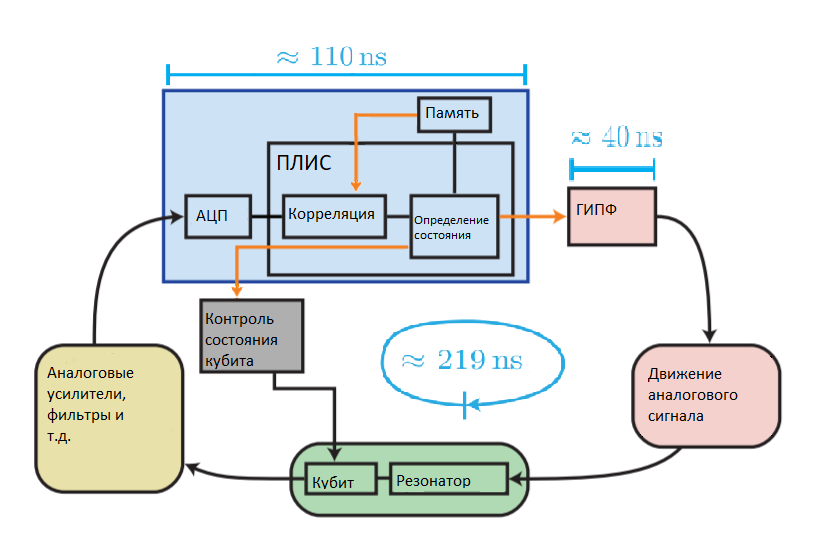
\includegraphics[width=0.7\linewidth]{pictures/feedback}
	\caption{Схема обратной связи}
	\label{fig:feedback}
\end{figure}

С помощью генератора сигналов произвольной формы на образец подаётся считывающий импульс, на выходе из образца он попадает в АЦП. По интерфейсу JESD204b он попадет в модуль ответственный за захват данных. Дополнительно в этот модуль был установлен линейный дискриминатор, подобный тому, что описан в (\ref{discr}). Этот дискриминатор считывает заранее записанные эталонные значения напряжения, соответствующие состояния $|0\rangle$ и $|1\rangle$, считает значение разности коэффициентов ковариации и в зависимости от величины этого значения принимает решение послать или не послать дополнительный сигнал на кубит. 

Как видно из схемы, на весь цикл уходит время порядка 200 нс, что существенно меньше времени релаксации. Использование быстрой обратной связи может быть использовано и в ряде других задач, таких как например передача классического ключа в алгоритме квантовой телепортации, выборочный контроль состояний одних кубитов, в зависимости от состояний других и т.д.




	\clearpage
	\begin{center}
	\large Выводы
\end{center}

\addcontentsline{toc}{section}{Выводы}

1. На основе методик машинного обучения разработан метод единовременного считывания квантового состояния сверхпроводящих кубитов; 

2. Разработана методика разделения ошибок приготовления и считывания квантовых состояний сверхпроводящих кубитов путём использования последовательности двух считывающих импульсов на основное состояние;

3. Создан программно-аппаратный комплекс, позволяющий проводить оцифровку и вычисление статистических параметров сигнала за сверхмалые времена (порядка сотен наносекунд);

4. На базе данного программно-аппаратного комплекса была реализована схема обратной связи для коррекции начального состояния сверхпроводящих кубитов и подготовки их к проведению квантовых алгоритмов.

	\clearpage 
	\addcontentsline{toc}{section}{Список использованных источников}

%\renewcommand*{\bibname}{Список использованных источников}

\renewcommand{\refname}{\filcenter Список использованных источников}
\bibliographystyle{sources/utfgost}
\bibliography{sources/Diplomas_references}

%Не смотрите туда, меня заставили :c
%\begin{center}
%	\large Список использованных источников
%\end{center}

%1\quad Feynman Richard P. Simulating with quantum computers // International Journal of Theoretical Physics. -- 1982. -- V.21. -- P.467--488

%2\quad Shor Peter W. Polynomial-Time Algorithms for Prime Factorization and Discrete Logarithms on a Quantum Computer // International Journal of Theoretical Physics. --1995. -- V.10. -- P.124--134

%3\quad Grover, Lov K. A fast quantum mechanical algorithm for database search // Proceedings of the twenty-eighth annual ACM symposium on Theory of computing. --1996. -- V.7. -- P.212--219

%4\quad Neumann, Von. Von Neumann's Contributions To Quantum Theory// International Journal of Theoretical Physics. -- 1957. -- V.4. -- P.95-99

%5\quad Feynman, R. P. and Vernon, F. L. The theory of a general quantum system interacting with a linear dissipative system // Annals of Physics. --1963. -- V.55. -- P.118--173

%6\quad Gu Xiu,  Kockum Anton Frisk and Miranowicz Adam et al. // Microwave photonics with superconducting quantum circuit // Physics Reports. --2017. -- V.102. -- P.1--102

%7\quad Budini Adri Open quantum system approach to single-molecule spectroscopy // Physical Review A - Atomic, Molecular, and Optical Physics. --2009. -- V.79. -- P.1--79

%8\quad Talkner Peter and Campisi Michele  Fluctuation theorems in driven open quantum systems // Journal of Statistical Mechanics: Theory and Experiment --2009. -- V.13. -- P.73--86

%9\quad Vool Uri and Devoret Michel Introduction to quantum electromagnetic circuits // International Journal of Circuit Theory and Applications --2008. -- V.43. -- P.40--83

%10\quad Gershenfeld Neil A and Chuang Isaac L Bulk Spin-Resonance Quantum Computation // Physics Reports. --1997. -- V.51. -- P.45-96

%11\quad Jaksch D.,Cirac J. I.  Zoller P. et al. Fast quantum gates for neutral atoms // Physical Review Letters. --2000. -- V.12. -- P.28--40

%12\quad Buluta Iulia, Ashhab Sahel and Nori, Franco Natural and artificial atoms for quantum computation // Reports on Progress in Physics. --2011. -- V.74. -- P.13--87

%13\quad Yan Fei, Gustavsson Simon, Kamal Archana et al. The flux qubit revisited to enhance coherence and reproducibility // Nature Communications. --2007. -- V.23. -- P.17--40

%14\quad Martinis John M. Superconducting phase qubits // Quantum Information Processing. --2001. -- V.17. -- P.1--17

%15\quad de Graaf S. E., Skacel S. T. Shaikhaidarov R. et al. Charge quantum interference device // Nature Physics. --2018. -- V.13. -- P.43--66
	
%16\quad Nakamura, Y., Pashkin, Yu A. and Tsai, J. S. Coherent control of macroscopic quantum states in a single-Cooper-pair box // Nature. --1999. -- V.10. -- P.23--33

%17\quad Shulga K. Coherent control of twin qubits // Nature Communication. --2017. -- V.13. -- P.33--46

%18\quad Wendin, G. and Shumeiko, V. S. Superconducting Quantum Circuits, Qubits and Computing // Nature Communication. -- 2005. -- V.8. -- P.30--38

%19\quad Koch Jens, Yu, Terri M. Gambetta Jay et al. Charge-insensitive qubit design derived from the Cooper pair box // Physical Review A - Atomic, Molecular, and Optical Physics. --2007. -- V.21. -- P.1--21

%20\quad Kleiner Reinhold and Koelle Dieter Superconducting Quantum Interference Devices : State of the Art and Applications //Nature Communications. --2011. -- V.31. -- P.10--21

%21\quad Wallraff A., Schuster, D. I. and Blais, A.  Approaching unit visibility for control of a superconducting qubit with dispersive readout //Physical Review Letters --2012. -- V.27. -- P.10--37

%22\quad Blais Alexandre, Huang Ren Shou, Wallraff Andreas et al.Cavity quantum electrodynamics for superconducting electrical circuits: An architecture for quantum computation //Physical Review A - Atomic, Molecular, and Optical Physics. --2004. -- V.48. -- P.22--70

%23\quad Wallraff A., Schuster, D. I. and Blais, A.  Approaching unit visibility for control of a superconducting qubit with dispersive readout //Physical Review Letters. --2012. -- V.27. -- P.10--37

%23\quad Clarke John and Wilhelm Frank K. Superconducting quantum bits // Nature. --2014. -- V.13. -- P.13--26

%24\quad Stammeier M., Garcia, S., Thiele T. Measuring the dispersive frequency shift of a rectangular microwave cavity induced by an ensemble of Rydberg atoms // Physical Review A - Atomic, Molecular, and Optical Physics. --2008. -- V.12. -- P.31--43

%25\quad Kox, A. J.The discovery of the Stark effect and its early theoretical explanations //Annalen der Physics. --2004. -- V.22. -- P.35--57

%26\quad Chen Yu, Sank D.,Omalley P. et al. Multiplexed dispersive readout of superconducting phase qubits //Applied Physics Letters. --2012. -- V.101. -- P.1--101

%27\quad Leng Xiang, Garcia-Barriocanal Javier and Bose Shameek Electrostatic control of the evolution from a superconducting phase to an insulating phase in ultrathin YBa2Cu3O7-x films //Physical Review Letters. --2011. -- V.13. -- P.13--26

%28\quad Magesan Easwar and Gambetta Jay M.Machine Learning for Discriminating Quantum Measurement Trajectories and Improving Readout //Physical Review Letters. --2015. -- V.10. -- P.23--33












	\clearpage
\end{document}